\documentclass[twoside]{book}

% Packages required by doxygen
\usepackage{calc}
\usepackage{doxygen}
\usepackage{graphicx}
\usepackage[utf8]{inputenc}
\usepackage{makeidx}
\usepackage{multicol}
\usepackage{multirow}
\usepackage{textcomp}
\usepackage[table]{xcolor}

% Font selection
\usepackage[T1]{fontenc}
\usepackage{mathptmx}
\usepackage[scaled=.90]{helvet}
\usepackage{courier}
\usepackage{amssymb}
\usepackage{sectsty}
\renewcommand{\familydefault}{\sfdefault}
\allsectionsfont{%
  \fontseries{bc}\selectfont%
  \color{darkgray}%
}
\renewcommand{\DoxyLabelFont}{%
  \fontseries{bc}\selectfont%
  \color{darkgray}%
}

% Page & text layout
\usepackage{geometry}
\geometry{%
  a4paper,%
  top=2.5cm,%
  bottom=2.5cm,%
  left=2.5cm,%
  right=2.5cm%
}
\tolerance=750
\hfuzz=15pt
\hbadness=750
\setlength{\emergencystretch}{15pt}
\setlength{\parindent}{0cm}
\setlength{\parskip}{0.2cm}
\makeatletter
\renewcommand{\paragraph}{%
  \@startsection{paragraph}{4}{0ex}{-1.0ex}{1.0ex}{%
    \normalfont\normalsize\bfseries\SS@parafont%
  }%
}
\renewcommand{\subparagraph}{%
  \@startsection{subparagraph}{5}{0ex}{-1.0ex}{1.0ex}{%
    \normalfont\normalsize\bfseries\SS@subparafont%
  }%
}
\makeatother

% Headers & footers
\usepackage{fancyhdr}
\pagestyle{fancyplain}
\fancyhead[LE]{\fancyplain{}{\bfseries\thepage}}
\fancyhead[CE]{\fancyplain{}{}}
\fancyhead[RE]{\fancyplain{}{\bfseries\leftmark}}
\fancyhead[LO]{\fancyplain{}{\bfseries\rightmark}}
\fancyhead[CO]{\fancyplain{}{}}
\fancyhead[RO]{\fancyplain{}{\bfseries\thepage}}
\fancyfoot[LE]{\fancyplain{}{}}
\fancyfoot[CE]{\fancyplain{}{}}
\fancyfoot[RE]{\fancyplain{}{\bfseries\scriptsize Generated on Mon Dec 16 2013 23\-:33\-:16 for R\-E\-S\-T Service by Doxygen }}
\fancyfoot[LO]{\fancyplain{}{\bfseries\scriptsize Generated on Mon Dec 16 2013 23\-:33\-:16 for R\-E\-S\-T Service by Doxygen }}
\fancyfoot[CO]{\fancyplain{}{}}
\fancyfoot[RO]{\fancyplain{}{}}
\renewcommand{\footrulewidth}{0.4pt}
\renewcommand{\chaptermark}[1]{%
  \markboth{#1}{}%
}
\renewcommand{\sectionmark}[1]{%
  \markright{\thesection\ #1}%
}

% Indices & bibliography
\usepackage{natbib}
\usepackage[titles]{tocloft}
\setcounter{tocdepth}{3}
\setcounter{secnumdepth}{5}
\makeindex

% Hyperlinks (required, but should be loaded last)
\usepackage{ifpdf}
\ifpdf
  \usepackage[pdftex,pagebackref=true]{hyperref}
\else
  \usepackage[ps2pdf,pagebackref=true]{hyperref}
\fi
\hypersetup{%
  colorlinks=true,%
  linkcolor=blue,%
  citecolor=blue,%
  unicode%
}

% Custom commands
\newcommand{\clearemptydoublepage}{%
  \newpage{\pagestyle{empty}\cleardoublepage}%
}


%===== C O N T E N T S =====

\begin{document}

% Titlepage & ToC
\hypersetup{pageanchor=false}
\pagenumbering{roman}
\begin{titlepage}
\vspace*{7cm}
\begin{center}%
{\Large R\-E\-S\-T Service \\[1ex]\large v.\-0.\-8 }\\
\vspace*{1cm}
{\large Generated by Doxygen 1.8.5}\\
\vspace*{0.5cm}
{\small Mon Dec 16 2013 23:33:16}\\
\end{center}
\end{titlepage}
\clearemptydoublepage
\tableofcontents
\clearemptydoublepage
\pagenumbering{arabic}
\hypersetup{pageanchor=true}

%--- Begin generated contents ---
\chapter{Namespace Index}
\section{Packages}
Here are the packages with brief descriptions (if available)\-:\begin{DoxyCompactList}
\item\contentsline{section}{\hyperlink{namespace_service_library}{Service\-Library} }{\pageref{namespace_service_library}}{}
\item\contentsline{section}{\hyperlink{namespace_service_library_1_1_database}{Service\-Library.\-Database} }{\pageref{namespace_service_library_1_1_database}}{}
\item\contentsline{section}{\hyperlink{namespace_windows_service}{Windows\-Service} }{\pageref{namespace_windows_service}}{}
\end{DoxyCompactList}

\chapter{Hierarchical Index}
\section{Class Hierarchy}
This inheritance list is sorted roughly, but not completely, alphabetically\-:\begin{DoxyCompactList}
\item \contentsline{section}{Service\-Library.\-Auth}{\pageref{class_service_library_1_1_auth}}{}
\item Db\-Context\begin{DoxyCompactList}
\item \contentsline{section}{Service\-Library.\-Database.\-Rest\-Entities}{\pageref{class_service_library_1_1_database_1_1_rest_entities}}{}
\end{DoxyCompactList}
\item \contentsline{section}{Service\-Library.\-Database.\-fleamarket\-\_\-addresses}{\pageref{class_service_library_1_1_database_1_1fleamarket__addresses}}{}
\item \contentsline{section}{Service\-Library.\-Database.\-fleamarket\-\_\-items}{\pageref{class_service_library_1_1_database_1_1fleamarket__items}}{}
\item \contentsline{section}{Service\-Library.\-Database.\-fleamarket\-\_\-openings}{\pageref{class_service_library_1_1_database_1_1fleamarket__openings}}{}
\item \contentsline{section}{Service\-Library.\-Database.\-fleamarket\-\_\-reviews}{\pageref{class_service_library_1_1_database_1_1fleamarket__reviews}}{}
\item \contentsline{section}{Service\-Library.\-Database.\-fleamarkets}{\pageref{class_service_library_1_1_database_1_1fleamarkets}}{}
\item Installer\begin{DoxyCompactList}
\item \contentsline{section}{Windows\-Service.\-Project\-Installer}{\pageref{class_windows_service_1_1_project_installer}}{}
\end{DoxyCompactList}
\item \contentsline{section}{Service\-Library.\-I\-Rest\-Service}{\pageref{interface_service_library_1_1_i_rest_service}}{}
\begin{DoxyCompactList}
\item \contentsline{section}{Service\-Library.\-Rest\-Service}{\pageref{class_service_library_1_1_rest_service}}{}
\end{DoxyCompactList}
\item \contentsline{section}{Windows\-Service.\-Program}{\pageref{class_windows_service_1_1_program}}{}
\item \contentsline{section}{Service\-Library.\-Response}{\pageref{class_service_library_1_1_response}}{}
\item Service\-Base\begin{DoxyCompactList}
\item \contentsline{section}{Windows\-Service.\-Service}{\pageref{class_windows_service_1_1_service}}{}
\end{DoxyCompactList}
\item \contentsline{section}{Service\-Library.\-Database.\-users}{\pageref{class_service_library_1_1_database_1_1users}}{}
\item \contentsline{section}{Service\-Library.\-Utility}{\pageref{class_service_library_1_1_utility}}{}
\item \contentsline{section}{Service\-Library.\-Wrapper}{\pageref{class_service_library_1_1_wrapper}}{}
\end{DoxyCompactList}

\chapter{Class Index}
\section{Class List}
Here are the classes, structs, unions and interfaces with brief descriptions\-:\begin{DoxyCompactList}
\item\contentsline{section}{\hyperlink{class_service_library_1_1_auth}{Service\-Library.\-Auth} \\*Class that handles user authentication calls towards database }{\pageref{class_service_library_1_1_auth}}{}
\item\contentsline{section}{\hyperlink{class_service_library_1_1_database_1_1fleamarket__addresses}{Service\-Library.\-Database.\-fleamarket\-\_\-addresses} }{\pageref{class_service_library_1_1_database_1_1fleamarket__addresses}}{}
\item\contentsline{section}{\hyperlink{class_service_library_1_1_database_1_1fleamarket__items}{Service\-Library.\-Database.\-fleamarket\-\_\-items} }{\pageref{class_service_library_1_1_database_1_1fleamarket__items}}{}
\item\contentsline{section}{\hyperlink{class_service_library_1_1_database_1_1fleamarket__openings}{Service\-Library.\-Database.\-fleamarket\-\_\-openings} }{\pageref{class_service_library_1_1_database_1_1fleamarket__openings}}{}
\item\contentsline{section}{\hyperlink{class_service_library_1_1_database_1_1fleamarket__reviews}{Service\-Library.\-Database.\-fleamarket\-\_\-reviews} }{\pageref{class_service_library_1_1_database_1_1fleamarket__reviews}}{}
\item\contentsline{section}{\hyperlink{class_service_library_1_1_database_1_1fleamarkets}{Service\-Library.\-Database.\-fleamarkets} }{\pageref{class_service_library_1_1_database_1_1fleamarkets}}{}
\item\contentsline{section}{\hyperlink{interface_service_library_1_1_i_rest_service}{Service\-Library.\-I\-Rest\-Service} \\*Interface for rest framework interfaced from the outside }{\pageref{interface_service_library_1_1_i_rest_service}}{}
\item\contentsline{section}{\hyperlink{class_windows_service_1_1_program}{Windows\-Service.\-Program} }{\pageref{class_windows_service_1_1_program}}{}
\item\contentsline{section}{\hyperlink{class_windows_service_1_1_project_installer}{Windows\-Service.\-Project\-Installer} }{\pageref{class_windows_service_1_1_project_installer}}{}
\item\contentsline{section}{\hyperlink{class_service_library_1_1_response}{Service\-Library.\-Response} \\*Class to handle response of the rest framework }{\pageref{class_service_library_1_1_response}}{}
\item\contentsline{section}{\hyperlink{class_service_library_1_1_database_1_1_rest_entities}{Service\-Library.\-Database.\-Rest\-Entities} }{\pageref{class_service_library_1_1_database_1_1_rest_entities}}{}
\item\contentsline{section}{\hyperlink{class_service_library_1_1_rest_service}{Service\-Library.\-Rest\-Service} }{\pageref{class_service_library_1_1_rest_service}}{}
\item\contentsline{section}{\hyperlink{class_windows_service_1_1_service}{Windows\-Service.\-Service} }{\pageref{class_windows_service_1_1_service}}{}
\item\contentsline{section}{\hyperlink{class_service_library_1_1_database_1_1users}{Service\-Library.\-Database.\-users} }{\pageref{class_service_library_1_1_database_1_1users}}{}
\item\contentsline{section}{\hyperlink{class_service_library_1_1_utility}{Service\-Library.\-Utility} \\*\hyperlink{class_service_library_1_1_utility}{Utility} class that serves functions that doesnt belong anywhere specific. }{\pageref{class_service_library_1_1_utility}}{}
\item\contentsline{section}{\hyperlink{class_service_library_1_1_wrapper}{Service\-Library.\-Wrapper} \\*\hyperlink{class_service_library_1_1_wrapper}{Wrapper} class which is used throughout to convert results to json output for rest framework }{\pageref{class_service_library_1_1_wrapper}}{}
\end{DoxyCompactList}

\chapter{Namespace Documentation}
\hypertarget{namespace_service_library}{\section{Package Service\-Library}
\label{namespace_service_library}\index{Service\-Library@{Service\-Library}}
}
\subsection*{Namespaces}
\begin{DoxyCompactItemize}
\item 
package \hyperlink{namespace_service_library_1_1_database}{Database}
\end{DoxyCompactItemize}
\subsection*{Classes}
\begin{DoxyCompactItemize}
\item 
class \hyperlink{class_service_library_1_1_auth}{Auth}
\begin{DoxyCompactList}\small\item\em Class that handles user authentication calls towards database \end{DoxyCompactList}\item 
interface \hyperlink{interface_service_library_1_1_i_rest_service}{I\-Rest\-Service}
\begin{DoxyCompactList}\small\item\em Interface for rest framework interfaced from the outside \end{DoxyCompactList}\item 
class \hyperlink{class_service_library_1_1_response}{Response}
\begin{DoxyCompactList}\small\item\em Class to handle response of the rest framework \end{DoxyCompactList}\item 
class \hyperlink{class_service_library_1_1_rest_service}{Rest\-Service}
\item 
class \hyperlink{class_service_library_1_1_utility}{Utility}
\begin{DoxyCompactList}\small\item\em \hyperlink{class_service_library_1_1_utility}{Utility} class that serves functions that doesnt belong anywhere specific. \end{DoxyCompactList}\item 
class \hyperlink{class_service_library_1_1_wrapper}{Wrapper}
\begin{DoxyCompactList}\small\item\em \hyperlink{class_service_library_1_1_wrapper}{Wrapper} class which is used throughout to convert results to json output for rest framework \end{DoxyCompactList}\end{DoxyCompactItemize}

\hypertarget{namespace_service_library_1_1_database}{\section{Package Service\-Library.\-Database}
\label{namespace_service_library_1_1_database}\index{Service\-Library.\-Database@{Service\-Library.\-Database}}
}
\subsection*{Classes}
\begin{DoxyCompactItemize}
\item 
class \hyperlink{class_service_library_1_1_database_1_1fleamarket__addresses}{fleamarket\-\_\-addresses}
\item 
class \hyperlink{class_service_library_1_1_database_1_1fleamarket__items}{fleamarket\-\_\-items}
\item 
class \hyperlink{class_service_library_1_1_database_1_1fleamarket__openings}{fleamarket\-\_\-openings}
\item 
class \hyperlink{class_service_library_1_1_database_1_1fleamarket__reviews}{fleamarket\-\_\-reviews}
\item 
class \hyperlink{class_service_library_1_1_database_1_1fleamarkets}{fleamarkets}
\item 
class \hyperlink{class_service_library_1_1_database_1_1_rest_entities}{Rest\-Entities}
\item 
class \hyperlink{class_service_library_1_1_database_1_1users}{users}
\end{DoxyCompactItemize}

\hypertarget{namespace_windows_service}{\section{Package Windows\-Service}
\label{namespace_windows_service}\index{Windows\-Service@{Windows\-Service}}
}
\subsection*{Classes}
\begin{DoxyCompactItemize}
\item 
class \hyperlink{class_windows_service_1_1_program}{Program}
\item 
class \hyperlink{class_windows_service_1_1_project_installer}{Project\-Installer}
\item 
class \hyperlink{class_windows_service_1_1_service}{Service}
\end{DoxyCompactItemize}

\chapter{Class Documentation}
\hypertarget{class_service_library_1_1_auth}{\section{Service\-Library.\-Auth Class Reference}
\label{class_service_library_1_1_auth}\index{Service\-Library.\-Auth@{Service\-Library.\-Auth}}
}


Class that handles user authentication calls towards database  


\subsection*{Static Public Member Functions}
\begin{DoxyCompactItemize}
\item 
static \hyperlink{class_service_library_1_1_wrapper}{Wrapper} \hyperlink{class_service_library_1_1_auth_a13db4b76836e33e52ab853b30289e149}{register} (string username, string password)
\begin{DoxyCompactList}\small\item\em Function registers a user with given username and password for the rest framework on the database \end{DoxyCompactList}\item 
static \hyperlink{class_service_library_1_1_wrapper}{Wrapper} \hyperlink{class_service_library_1_1_auth_a6bcc9764de39110acf53dc03257296fc}{login} (string username, string password)
\begin{DoxyCompactList}\small\item\em Function checks whether a user with given username and password exists and is valid \end{DoxyCompactList}\end{DoxyCompactItemize}


\subsection{Detailed Description}
Class that handles user authentication calls towards database 



\subsection{Member Function Documentation}
\hypertarget{class_service_library_1_1_auth_a6bcc9764de39110acf53dc03257296fc}{\index{Service\-Library\-::\-Auth@{Service\-Library\-::\-Auth}!login@{login}}
\index{login@{login}!ServiceLibrary::Auth@{Service\-Library\-::\-Auth}}
\subsubsection[{login}]{\setlength{\rightskip}{0pt plus 5cm}static {\bf Wrapper} Service\-Library.\-Auth.\-login (
\begin{DoxyParamCaption}
\item[{string}]{username, }
\item[{string}]{password}
\end{DoxyParamCaption}
)\hspace{0.3cm}{\ttfamily [static]}}}\label{class_service_library_1_1_auth_a6bcc9764de39110acf53dc03257296fc}


Function checks whether a user with given username and password exists and is valid 


\begin{DoxyParams}{Parameters}
{\em username} & User username string\\
\hline
{\em password} & User password string\\
\hline
\end{DoxyParams}
\begin{DoxyReturn}{Returns}
Returns wrapper with status and error code
\end{DoxyReturn}
\hypertarget{class_service_library_1_1_auth_a13db4b76836e33e52ab853b30289e149}{\index{Service\-Library\-::\-Auth@{Service\-Library\-::\-Auth}!register@{register}}
\index{register@{register}!ServiceLibrary::Auth@{Service\-Library\-::\-Auth}}
\subsubsection[{register}]{\setlength{\rightskip}{0pt plus 5cm}static {\bf Wrapper} Service\-Library.\-Auth.\-register (
\begin{DoxyParamCaption}
\item[{string}]{username, }
\item[{string}]{password}
\end{DoxyParamCaption}
)\hspace{0.3cm}{\ttfamily [static]}}}\label{class_service_library_1_1_auth_a13db4b76836e33e52ab853b30289e149}


Function registers a user with given username and password for the rest framework on the database 


\begin{DoxyParams}{Parameters}
{\em username} & Users username string\\
\hline
{\em password} & Users password string\\
\hline
\end{DoxyParams}
\begin{DoxyReturn}{Returns}
Returns a class wrapper with user info, error code and whether it succeded
\end{DoxyReturn}


The documentation for this class was generated from the following file\-:\begin{DoxyCompactItemize}
\item 
Service\-Library/auth.\-cs\end{DoxyCompactItemize}

\hypertarget{class_service_library_1_1_database_1_1fleamarket__addresses}{\section{Service\-Library.\-Database.\-fleamarket\-\_\-addresses Class Reference}
\label{class_service_library_1_1_database_1_1fleamarket__addresses}\index{Service\-Library.\-Database.\-fleamarket\-\_\-addresses@{Service\-Library.\-Database.\-fleamarket\-\_\-addresses}}
}
\subsection*{Properties}
\begin{DoxyCompactItemize}
\item 
\hypertarget{class_service_library_1_1_database_1_1fleamarket__addresses_a4da474708fde2ff8fc67fb69d79f9ffb}{int {\bfseries id}\hspace{0.3cm}{\ttfamily  \mbox{[}get, set\mbox{]}}}\label{class_service_library_1_1_database_1_1fleamarket__addresses_a4da474708fde2ff8fc67fb69d79f9ffb}

\item 
\hypertarget{class_service_library_1_1_database_1_1fleamarket__addresses_ac19818b3701f6637044ed6628070e782}{string {\bfseries city}\hspace{0.3cm}{\ttfamily  \mbox{[}get, set\mbox{]}}}\label{class_service_library_1_1_database_1_1fleamarket__addresses_ac19818b3701f6637044ed6628070e782}

\item 
\hypertarget{class_service_library_1_1_database_1_1fleamarket__addresses_a1fc1a22790374ec43421b742a692212f}{string {\bfseries street}\hspace{0.3cm}{\ttfamily  \mbox{[}get, set\mbox{]}}}\label{class_service_library_1_1_database_1_1fleamarket__addresses_a1fc1a22790374ec43421b742a692212f}

\item 
\hypertarget{class_service_library_1_1_database_1_1fleamarket__addresses_a56ea47ce8098aa8a8cea741fe9134279}{string {\bfseries postcode}\hspace{0.3cm}{\ttfamily  \mbox{[}get, set\mbox{]}}}\label{class_service_library_1_1_database_1_1fleamarket__addresses_a56ea47ce8098aa8a8cea741fe9134279}

\item 
\hypertarget{class_service_library_1_1_database_1_1fleamarket__addresses_a874d8519eb5fe9fe742e822ce834cd94}{float {\bfseries latitude}\hspace{0.3cm}{\ttfamily  \mbox{[}get, set\mbox{]}}}\label{class_service_library_1_1_database_1_1fleamarket__addresses_a874d8519eb5fe9fe742e822ce834cd94}

\item 
\hypertarget{class_service_library_1_1_database_1_1fleamarket__addresses_a884d58e226129da850fce34c4418dd14}{float {\bfseries longitude}\hspace{0.3cm}{\ttfamily  \mbox{[}get, set\mbox{]}}}\label{class_service_library_1_1_database_1_1fleamarket__addresses_a884d58e226129da850fce34c4418dd14}

\item 
\hypertarget{class_service_library_1_1_database_1_1fleamarket__addresses_ade7ccd5ff7d9f6bb4056b23316aea317}{virtual I\-Collection$<$ \hyperlink{class_service_library_1_1_database_1_1fleamarkets}{fleamarkets} $>$ {\bfseries fleamarkets}\hspace{0.3cm}{\ttfamily  \mbox{[}get, set\mbox{]}}}\label{class_service_library_1_1_database_1_1fleamarket__addresses_ade7ccd5ff7d9f6bb4056b23316aea317}

\end{DoxyCompactItemize}


The documentation for this class was generated from the following file\-:\begin{DoxyCompactItemize}
\item 
Service\-Library/\-Database/fleamarket\-\_\-addresses.\-cs\end{DoxyCompactItemize}

\hypertarget{class_service_library_1_1_database_1_1fleamarket__items}{\section{Service\-Library.\-Database.\-fleamarket\-\_\-items Class Reference}
\label{class_service_library_1_1_database_1_1fleamarket__items}\index{Service\-Library.\-Database.\-fleamarket\-\_\-items@{Service\-Library.\-Database.\-fleamarket\-\_\-items}}
}
\subsection*{Properties}
\begin{DoxyCompactItemize}
\item 
\hypertarget{class_service_library_1_1_database_1_1fleamarket__items_ad3e7996326f63391feca9b26e96eec5c}{int {\bfseries id}\hspace{0.3cm}{\ttfamily  \mbox{[}get, set\mbox{]}}}\label{class_service_library_1_1_database_1_1fleamarket__items_ad3e7996326f63391feca9b26e96eec5c}

\item 
\hypertarget{class_service_library_1_1_database_1_1fleamarket__items_a248368019fc66df572defd04099b1990}{string {\bfseries name}\hspace{0.3cm}{\ttfamily  \mbox{[}get, set\mbox{]}}}\label{class_service_library_1_1_database_1_1fleamarket__items_a248368019fc66df572defd04099b1990}

\item 
\hypertarget{class_service_library_1_1_database_1_1fleamarket__items_a3529ee135423e926c89e355d5d00d592}{virtual I\-Collection$<$ \hyperlink{class_service_library_1_1_database_1_1fleamarkets}{fleamarkets} $>$ {\bfseries fleamarkets}\hspace{0.3cm}{\ttfamily  \mbox{[}get, set\mbox{]}}}\label{class_service_library_1_1_database_1_1fleamarket__items_a3529ee135423e926c89e355d5d00d592}

\end{DoxyCompactItemize}


The documentation for this class was generated from the following file\-:\begin{DoxyCompactItemize}
\item 
Service\-Library/\-Database/fleamarket\-\_\-items.\-cs\end{DoxyCompactItemize}

\hypertarget{class_service_library_1_1_database_1_1fleamarket__openings}{\section{Service\-Library.\-Database.\-fleamarket\-\_\-openings Class Reference}
\label{class_service_library_1_1_database_1_1fleamarket__openings}\index{Service\-Library.\-Database.\-fleamarket\-\_\-openings@{Service\-Library.\-Database.\-fleamarket\-\_\-openings}}
}
\subsection*{Properties}
\begin{DoxyCompactItemize}
\item 
\hypertarget{class_service_library_1_1_database_1_1fleamarket__openings_a68f0fb19119daba13ad2bd0d17155fcb}{int {\bfseries id}\hspace{0.3cm}{\ttfamily  \mbox{[}get, set\mbox{]}}}\label{class_service_library_1_1_database_1_1fleamarket__openings_a68f0fb19119daba13ad2bd0d17155fcb}

\item 
\hypertarget{class_service_library_1_1_database_1_1fleamarket__openings_a9995107aab65b60e7bed709246450828}{System.\-Date\-Time {\bfseries from}\hspace{0.3cm}{\ttfamily  \mbox{[}get, set\mbox{]}}}\label{class_service_library_1_1_database_1_1fleamarket__openings_a9995107aab65b60e7bed709246450828}

\item 
\hypertarget{class_service_library_1_1_database_1_1fleamarket__openings_a58b2a047a2f688ba8f8674df0bee7b56}{System.\-Date\-Time {\bfseries to}\hspace{0.3cm}{\ttfamily  \mbox{[}get, set\mbox{]}}}\label{class_service_library_1_1_database_1_1fleamarket__openings_a58b2a047a2f688ba8f8674df0bee7b56}

\item 
\hypertarget{class_service_library_1_1_database_1_1fleamarket__openings_a0d643bff256d4a1af4a90799f4f58f21}{int {\bfseries fleamarkets\-\_\-id}\hspace{0.3cm}{\ttfamily  \mbox{[}get, set\mbox{]}}}\label{class_service_library_1_1_database_1_1fleamarket__openings_a0d643bff256d4a1af4a90799f4f58f21}

\item 
\hypertarget{class_service_library_1_1_database_1_1fleamarket__openings_a7f8f71660f7189995743d9cd968081f5}{string {\bfseries description}\hspace{0.3cm}{\ttfamily  \mbox{[}get, set\mbox{]}}}\label{class_service_library_1_1_database_1_1fleamarket__openings_a7f8f71660f7189995743d9cd968081f5}

\item 
\hypertarget{class_service_library_1_1_database_1_1fleamarket__openings_ad8631cd16f192583e3381d8deb7bed35}{virtual \hyperlink{class_service_library_1_1_database_1_1fleamarkets}{fleamarkets} {\bfseries fleamarkets}\hspace{0.3cm}{\ttfamily  \mbox{[}get, set\mbox{]}}}\label{class_service_library_1_1_database_1_1fleamarket__openings_ad8631cd16f192583e3381d8deb7bed35}

\end{DoxyCompactItemize}


The documentation for this class was generated from the following file\-:\begin{DoxyCompactItemize}
\item 
Service\-Library/\-Database/fleamarket\-\_\-openings.\-cs\end{DoxyCompactItemize}

\hypertarget{class_service_library_1_1_database_1_1fleamarket__reviews}{\section{Service\-Library.\-Database.\-fleamarket\-\_\-reviews Class Reference}
\label{class_service_library_1_1_database_1_1fleamarket__reviews}\index{Service\-Library.\-Database.\-fleamarket\-\_\-reviews@{Service\-Library.\-Database.\-fleamarket\-\_\-reviews}}
}
\subsection*{Properties}
\begin{DoxyCompactItemize}
\item 
\hypertarget{class_service_library_1_1_database_1_1fleamarket__reviews_ac0563ebf354abef70816c8adaf5cc7a6}{int {\bfseries users\-\_\-id}\hspace{0.3cm}{\ttfamily  \mbox{[}get, set\mbox{]}}}\label{class_service_library_1_1_database_1_1fleamarket__reviews_ac0563ebf354abef70816c8adaf5cc7a6}

\item 
\hypertarget{class_service_library_1_1_database_1_1fleamarket__reviews_a061da2fd1f910f5374036ee020e5e74f}{int {\bfseries fleamarkets\-\_\-id}\hspace{0.3cm}{\ttfamily  \mbox{[}get, set\mbox{]}}}\label{class_service_library_1_1_database_1_1fleamarket__reviews_a061da2fd1f910f5374036ee020e5e74f}

\item 
\hypertarget{class_service_library_1_1_database_1_1fleamarket__reviews_a6b4b2e9f2a3f0e28f8351b5a1471c9b6}{string {\bfseries text}\hspace{0.3cm}{\ttfamily  \mbox{[}get, set\mbox{]}}}\label{class_service_library_1_1_database_1_1fleamarket__reviews_a6b4b2e9f2a3f0e28f8351b5a1471c9b6}

\item 
\hypertarget{class_service_library_1_1_database_1_1fleamarket__reviews_ab5d4dc951343075041184af86506bd3d}{int {\bfseries stars}\hspace{0.3cm}{\ttfamily  \mbox{[}get, set\mbox{]}}}\label{class_service_library_1_1_database_1_1fleamarket__reviews_ab5d4dc951343075041184af86506bd3d}

\item 
\hypertarget{class_service_library_1_1_database_1_1fleamarket__reviews_ab1178ba69003c5b0e48f3a4f9ec844e3}{virtual \hyperlink{class_service_library_1_1_database_1_1fleamarkets}{fleamarkets} {\bfseries fleamarkets}\hspace{0.3cm}{\ttfamily  \mbox{[}get, set\mbox{]}}}\label{class_service_library_1_1_database_1_1fleamarket__reviews_ab1178ba69003c5b0e48f3a4f9ec844e3}

\item 
\hypertarget{class_service_library_1_1_database_1_1fleamarket__reviews_a618c9484d895bf9636e75cd32e55f93e}{virtual \hyperlink{class_service_library_1_1_database_1_1users}{users} {\bfseries users}\hspace{0.3cm}{\ttfamily  \mbox{[}get, set\mbox{]}}}\label{class_service_library_1_1_database_1_1fleamarket__reviews_a618c9484d895bf9636e75cd32e55f93e}

\end{DoxyCompactItemize}


The documentation for this class was generated from the following file\-:\begin{DoxyCompactItemize}
\item 
Service\-Library/\-Database/fleamarket\-\_\-reviews.\-cs\end{DoxyCompactItemize}

\hypertarget{class_service_library_1_1_database_1_1fleamarkets}{\section{Service\-Library.\-Database.\-fleamarkets Class Reference}
\label{class_service_library_1_1_database_1_1fleamarkets}\index{Service\-Library.\-Database.\-fleamarkets@{Service\-Library.\-Database.\-fleamarkets}}
}
\subsection*{Properties}
\begin{DoxyCompactItemize}
\item 
\hypertarget{class_service_library_1_1_database_1_1fleamarkets_a79402a398f6201e1fdef2e793bd0e908}{int {\bfseries id}\hspace{0.3cm}{\ttfamily  \mbox{[}get, set\mbox{]}}}\label{class_service_library_1_1_database_1_1fleamarkets_a79402a398f6201e1fdef2e793bd0e908}

\item 
\hypertarget{class_service_library_1_1_database_1_1fleamarkets_af75b9ced1933c6851dd7492be767f022}{string {\bfseries name}\hspace{0.3cm}{\ttfamily  \mbox{[}get, set\mbox{]}}}\label{class_service_library_1_1_database_1_1fleamarkets_af75b9ced1933c6851dd7492be767f022}

\item 
\hypertarget{class_service_library_1_1_database_1_1fleamarkets_ae3b43e66b8e4b6c186d390eef4c53852}{string {\bfseries description}\hspace{0.3cm}{\ttfamily  \mbox{[}get, set\mbox{]}}}\label{class_service_library_1_1_database_1_1fleamarkets_ae3b43e66b8e4b6c186d390eef4c53852}

\item 
\hypertarget{class_service_library_1_1_database_1_1fleamarkets_a9b484467c018f0edc249b520962b29a0}{string {\bfseries logo}\hspace{0.3cm}{\ttfamily  \mbox{[}get, set\mbox{]}}}\label{class_service_library_1_1_database_1_1fleamarkets_a9b484467c018f0edc249b520962b29a0}

\item 
\hypertarget{class_service_library_1_1_database_1_1fleamarkets_a7620eaed0bd301443a852956d454fe8f}{System.\-Date\-Time {\bfseries created\-\_\-on}\hspace{0.3cm}{\ttfamily  \mbox{[}get, set\mbox{]}}}\label{class_service_library_1_1_database_1_1fleamarkets_a7620eaed0bd301443a852956d454fe8f}

\item 
\hypertarget{class_service_library_1_1_database_1_1fleamarkets_a60849ff47691e46bbb71b52fc77e9ca1}{System.\-Date\-Time {\bfseries modified\-\_\-on}\hspace{0.3cm}{\ttfamily  \mbox{[}get, set\mbox{]}}}\label{class_service_library_1_1_database_1_1fleamarkets_a60849ff47691e46bbb71b52fc77e9ca1}

\item 
\hypertarget{class_service_library_1_1_database_1_1fleamarkets_a75338667e9a7769e38fe4a56dbf44f7a}{string {\bfseries category}\hspace{0.3cm}{\ttfamily  \mbox{[}get, set\mbox{]}}}\label{class_service_library_1_1_database_1_1fleamarkets_a75338667e9a7769e38fe4a56dbf44f7a}

\item 
\hypertarget{class_service_library_1_1_database_1_1fleamarkets_a4993a3de73fa86d4a3b9bc64eb7a9196}{int {\bfseries fleamarket\-\_\-addresses\-\_\-id}\hspace{0.3cm}{\ttfamily  \mbox{[}get, set\mbox{]}}}\label{class_service_library_1_1_database_1_1fleamarkets_a4993a3de73fa86d4a3b9bc64eb7a9196}

\item 
\hypertarget{class_service_library_1_1_database_1_1fleamarkets_a2b575f72b3e27ec877fa23725aa8c02a}{int {\bfseries users\-\_\-id}\hspace{0.3cm}{\ttfamily  \mbox{[}get, set\mbox{]}}}\label{class_service_library_1_1_database_1_1fleamarkets_a2b575f72b3e27ec877fa23725aa8c02a}

\item 
\hypertarget{class_service_library_1_1_database_1_1fleamarkets_a54be2b30ee83fef68ede7a892283fd40}{virtual \hyperlink{class_service_library_1_1_database_1_1fleamarket__addresses}{fleamarket\-\_\-addresses} {\bfseries fleamarket\-\_\-addresses}\hspace{0.3cm}{\ttfamily  \mbox{[}get, set\mbox{]}}}\label{class_service_library_1_1_database_1_1fleamarkets_a54be2b30ee83fef68ede7a892283fd40}

\item 
\hypertarget{class_service_library_1_1_database_1_1fleamarkets_a3cdee86a201bce680debc521fd7615d7}{virtual I\-Collection\\*
$<$ \hyperlink{class_service_library_1_1_database_1_1fleamarket__openings}{fleamarket\-\_\-openings} $>$ {\bfseries fleamarket\-\_\-openings}\hspace{0.3cm}{\ttfamily  \mbox{[}get, set\mbox{]}}}\label{class_service_library_1_1_database_1_1fleamarkets_a3cdee86a201bce680debc521fd7615d7}

\item 
\hypertarget{class_service_library_1_1_database_1_1fleamarkets_a4f3f79c7b961e664e7d92fa2a7c112aa}{virtual I\-Collection\\*
$<$ \hyperlink{class_service_library_1_1_database_1_1fleamarket__reviews}{fleamarket\-\_\-reviews} $>$ {\bfseries fleamarket\-\_\-reviews}\hspace{0.3cm}{\ttfamily  \mbox{[}get, set\mbox{]}}}\label{class_service_library_1_1_database_1_1fleamarkets_a4f3f79c7b961e664e7d92fa2a7c112aa}

\item 
\hypertarget{class_service_library_1_1_database_1_1fleamarkets_a62281e43603d4a180857b3df05e7d8c7}{virtual \hyperlink{class_service_library_1_1_database_1_1users}{users} {\bfseries users}\hspace{0.3cm}{\ttfamily  \mbox{[}get, set\mbox{]}}}\label{class_service_library_1_1_database_1_1fleamarkets_a62281e43603d4a180857b3df05e7d8c7}

\item 
\hypertarget{class_service_library_1_1_database_1_1fleamarkets_ae3be6ec0aa7a2aa5dba034146d75886d}{virtual I\-Collection\\*
$<$ \hyperlink{class_service_library_1_1_database_1_1fleamarket__items}{fleamarket\-\_\-items} $>$ {\bfseries fleamarket\-\_\-items}\hspace{0.3cm}{\ttfamily  \mbox{[}get, set\mbox{]}}}\label{class_service_library_1_1_database_1_1fleamarkets_ae3be6ec0aa7a2aa5dba034146d75886d}

\end{DoxyCompactItemize}


The documentation for this class was generated from the following file\-:\begin{DoxyCompactItemize}
\item 
Service\-Library/\-Database/fleamarkets.\-cs\end{DoxyCompactItemize}

\hypertarget{interface_service_library_1_1_i_rest_service}{\section{Service\-Library.\-I\-Rest\-Service Interface Reference}
\label{interface_service_library_1_1_i_rest_service}\index{Service\-Library.\-I\-Rest\-Service@{Service\-Library.\-I\-Rest\-Service}}
}


Interface for rest framework interfaced from the outside  




Inheritance diagram for Service\-Library.\-I\-Rest\-Service\-:\nopagebreak
\begin{figure}[H]
\begin{center}
\leavevmode
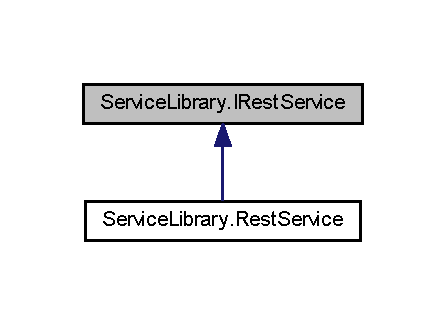
\includegraphics[width=214pt]{interface_service_library_1_1_i_rest_service__inherit__graph}
\end{center}
\end{figure}
\subsection*{Public Member Functions}
\begin{DoxyCompactItemize}
\item 
Stream \hyperlink{interface_service_library_1_1_i_rest_service_ad6d9e2dcc4d575310586390fa144d181}{fleamarket\-List} ()
\begin{DoxyCompactList}\small\item\em Function that shows all fleamarkets \end{DoxyCompactList}\item 
Stream \hyperlink{interface_service_library_1_1_i_rest_service_af1be4751f78a02a57e702a69054632cc}{fleamarket\-Description} (string id)
\begin{DoxyCompactList}\small\item\em Function that gets info about a specific market \end{DoxyCompactList}\item 
Stream \hyperlink{interface_service_library_1_1_i_rest_service_a54317be38e33419acaba46e8ba6a0958}{create\-Flea\-Market} (string username, string password, string name, string description, string logo, string category, string city, string street, string postcode, string latitude, string longitude)
\begin{DoxyCompactList}\small\item\em Creates a fleamarket on the database if authorised for it \end{DoxyCompactList}\item 
Stream \hyperlink{interface_service_library_1_1_i_rest_service_a6a7bcc09960ff24c5ce779e7be7d4ddb}{update\-Flea\-Market} (string username, string password, string fleamarket\-Id, string name, string description, string logo, string category, string city, string street, string postcode, string latitude, string longitude)
\begin{DoxyCompactList}\small\item\em Updates a certain fleamarket if authorised for it \end{DoxyCompactList}\item 
Stream \hyperlink{interface_service_library_1_1_i_rest_service_ab1f44acad37127065148c804d03fc36f}{delete\-Flea\-Market} (string username, string password, string fleamarket\-Id)
\begin{DoxyCompactList}\small\item\em Function that deletes a certain fleamarket if authorised for it \end{DoxyCompactList}\item 
Stream \hyperlink{interface_service_library_1_1_i_rest_service_a8da12dfeb7d26f50c935c17ed4969ef8}{create\-Opening} (string username, string password, string fleamarket\-Id, string from, string to, string description)
\begin{DoxyCompactList}\small\item\em Function that creates fleamarket openings if authorised for it \end{DoxyCompactList}\item 
Stream \hyperlink{interface_service_library_1_1_i_rest_service_aff55a9fbcda58a0830319982233420b8}{update\-Opening} (string username, string password, string opening\-Id, string from, string to, string description)
\begin{DoxyCompactList}\small\item\em Function that updates an existing opening if authorised for it \end{DoxyCompactList}\item 
Stream \hyperlink{interface_service_library_1_1_i_rest_service_a4bfa508142405715bb37792073c43eb2}{delete\-Opening} (string username, string password, string opening\-Id)
\begin{DoxyCompactList}\small\item\em Function that deletes an existing opening if authorised for it \end{DoxyCompactList}\item 
Stream \hyperlink{interface_service_library_1_1_i_rest_service_ae566a85d019d87c013ed069b381e59ee}{register} (string username, string password)
\begin{DoxyCompactList}\small\item\em Function that registers a user with given parameters \end{DoxyCompactList}\item 
Stream \hyperlink{interface_service_library_1_1_i_rest_service_aa0ee715b0c69f4c024ede0d91939c4a2}{login} (string username, string password)
\begin{DoxyCompactList}\small\item\em Function that checks if a username/password is a valid user \end{DoxyCompactList}\item 
Stream \hyperlink{interface_service_library_1_1_i_rest_service_a925656ba45a706648af391a00733e45f}{create\-Review} (string username, string password, string fleamarket\-Id, string stars, string text)
\begin{DoxyCompactList}\small\item\em Function to create review of a fleamarket, if authorised \end{DoxyCompactList}\item 
Stream \hyperlink{interface_service_library_1_1_i_rest_service_a8d80e4dac07cf691bc685c1944192f22}{update\-Review} (string username, string password, string fleamarket\-Id, string stars, string text)
\begin{DoxyCompactList}\small\item\em Function to update an existing review if authorised \end{DoxyCompactList}\item 
Stream \hyperlink{interface_service_library_1_1_i_rest_service_ae8340be9ca2f22dc5e3e93e7d2786c85}{delete\-Review} (string username, string password, string fleamarket\-Id)
\begin{DoxyCompactList}\small\item\em Function to delete existing reviews if authorised \end{DoxyCompactList}\end{DoxyCompactItemize}


\subsection{Detailed Description}
Interface for rest framework interfaced from the outside 



\subsection{Member Function Documentation}
\hypertarget{interface_service_library_1_1_i_rest_service_a54317be38e33419acaba46e8ba6a0958}{\index{Service\-Library\-::\-I\-Rest\-Service@{Service\-Library\-::\-I\-Rest\-Service}!create\-Flea\-Market@{create\-Flea\-Market}}
\index{create\-Flea\-Market@{create\-Flea\-Market}!ServiceLibrary::IRestService@{Service\-Library\-::\-I\-Rest\-Service}}
\subsubsection[{create\-Flea\-Market}]{\setlength{\rightskip}{0pt plus 5cm}Stream Service\-Library.\-I\-Rest\-Service.\-create\-Flea\-Market (
\begin{DoxyParamCaption}
\item[{string}]{username, }
\item[{string}]{password, }
\item[{string}]{name, }
\item[{string}]{description, }
\item[{string}]{logo, }
\item[{string}]{category, }
\item[{string}]{city, }
\item[{string}]{street, }
\item[{string}]{postcode, }
\item[{string}]{latitude, }
\item[{string}]{longitude}
\end{DoxyParamCaption}
)}}\label{interface_service_library_1_1_i_rest_service_a54317be38e33419acaba46e8ba6a0958}


Creates a fleamarket on the database if authorised for it 


\begin{DoxyParams}{Parameters}
{\em username} & Username of the user that wanna add market\\
\hline
{\em password} & Password of the user that wanna add market\\
\hline
{\em name} & Name of the fleamarket\\
\hline
{\em description} & Description of the fleamarket\\
\hline
{\em logo} & Logo of the fleamarket\\
\hline
{\em category} & Category of the fleamarket\\
\hline
{\em city} & City of the fleamarket\\
\hline
{\em street} & Street of the fleamarket\\
\hline
{\em postcode} & Postcode of the fleamarket\\
\hline
{\em latitude} & Latitude of the fleamarket\\
\hline
{\em longitude} & Longitude of the fleamarket\\
\hline
\end{DoxyParams}
\begin{DoxyReturn}{Returns}
J\-S\-O\-N of a wrapper with status
\end{DoxyReturn}


Implemented in \hyperlink{class_service_library_1_1_rest_service_a39a86dadc6525bee03594f583acff2da}{Service\-Library.\-Rest\-Service}.

\hypertarget{interface_service_library_1_1_i_rest_service_a8da12dfeb7d26f50c935c17ed4969ef8}{\index{Service\-Library\-::\-I\-Rest\-Service@{Service\-Library\-::\-I\-Rest\-Service}!create\-Opening@{create\-Opening}}
\index{create\-Opening@{create\-Opening}!ServiceLibrary::IRestService@{Service\-Library\-::\-I\-Rest\-Service}}
\subsubsection[{create\-Opening}]{\setlength{\rightskip}{0pt plus 5cm}Stream Service\-Library.\-I\-Rest\-Service.\-create\-Opening (
\begin{DoxyParamCaption}
\item[{string}]{username, }
\item[{string}]{password, }
\item[{string}]{fleamarket\-Id, }
\item[{string}]{from, }
\item[{string}]{to, }
\item[{string}]{description}
\end{DoxyParamCaption}
)}}\label{interface_service_library_1_1_i_rest_service_a8da12dfeb7d26f50c935c17ed4969ef8}


Function that creates fleamarket openings if authorised for it 


\begin{DoxyParams}{Parameters}
{\em username} & Username of the user wanting to add opening\\
\hline
{\em password} & Password of the user wanting to add opening\\
\hline
{\em fleamarket\-Id} & Id of the fleamarket to add opening\\
\hline
{\em from} & Datetime of the from time\\
\hline
{\em to} & Datetime of the to time\\
\hline
{\em description} & Description of the time\\
\hline
\end{DoxyParams}
\begin{DoxyReturn}{Returns}
J\-S\-O\-N of a wrapper with status
\end{DoxyReturn}


Implemented in \hyperlink{class_service_library_1_1_rest_service_a4d3293e03679b4d959f342308da43b1f}{Service\-Library.\-Rest\-Service}.

\hypertarget{interface_service_library_1_1_i_rest_service_a925656ba45a706648af391a00733e45f}{\index{Service\-Library\-::\-I\-Rest\-Service@{Service\-Library\-::\-I\-Rest\-Service}!create\-Review@{create\-Review}}
\index{create\-Review@{create\-Review}!ServiceLibrary::IRestService@{Service\-Library\-::\-I\-Rest\-Service}}
\subsubsection[{create\-Review}]{\setlength{\rightskip}{0pt plus 5cm}Stream Service\-Library.\-I\-Rest\-Service.\-create\-Review (
\begin{DoxyParamCaption}
\item[{string}]{username, }
\item[{string}]{password, }
\item[{string}]{fleamarket\-Id, }
\item[{string}]{stars, }
\item[{string}]{text}
\end{DoxyParamCaption}
)}}\label{interface_service_library_1_1_i_rest_service_a925656ba45a706648af391a00733e45f}


Function to create review of a fleamarket, if authorised 


\begin{DoxyParams}{Parameters}
{\em username} & Username of the user wanting to create review\\
\hline
{\em password} & Password of the user wanting to create review\\
\hline
{\em fleamarket\-Id} & Id of fleamarket to add review\\
\hline
{\em stars} & Amount of stars for review\\
\hline
{\em text} & Text for the review\\
\hline
\end{DoxyParams}
\begin{DoxyReturn}{Returns}
J\-S\-O\-N of a wrapper with status
\end{DoxyReturn}


Implemented in \hyperlink{class_service_library_1_1_rest_service_a0121954034b57e8947b9c5ce65479f65}{Service\-Library.\-Rest\-Service}.

\hypertarget{interface_service_library_1_1_i_rest_service_ab1f44acad37127065148c804d03fc36f}{\index{Service\-Library\-::\-I\-Rest\-Service@{Service\-Library\-::\-I\-Rest\-Service}!delete\-Flea\-Market@{delete\-Flea\-Market}}
\index{delete\-Flea\-Market@{delete\-Flea\-Market}!ServiceLibrary::IRestService@{Service\-Library\-::\-I\-Rest\-Service}}
\subsubsection[{delete\-Flea\-Market}]{\setlength{\rightskip}{0pt plus 5cm}Stream Service\-Library.\-I\-Rest\-Service.\-delete\-Flea\-Market (
\begin{DoxyParamCaption}
\item[{string}]{username, }
\item[{string}]{password, }
\item[{string}]{fleamarket\-Id}
\end{DoxyParamCaption}
)}}\label{interface_service_library_1_1_i_rest_service_ab1f44acad37127065148c804d03fc36f}


Function that deletes a certain fleamarket if authorised for it 


\begin{DoxyParams}{Parameters}
{\em username} & Username of the user wanting to delete a market\\
\hline
{\em password} & Password of the user wanting to delete a market\\
\hline
{\em fleamarket\-Id} & Id of the market to be deleted\\
\hline
\end{DoxyParams}
\begin{DoxyReturn}{Returns}
J\-S\-O\-N of a wrapper with status
\end{DoxyReturn}


Implemented in \hyperlink{class_service_library_1_1_rest_service_ab502a53d2f520a2b43803a10cb8a93d2}{Service\-Library.\-Rest\-Service}.

\hypertarget{interface_service_library_1_1_i_rest_service_a4bfa508142405715bb37792073c43eb2}{\index{Service\-Library\-::\-I\-Rest\-Service@{Service\-Library\-::\-I\-Rest\-Service}!delete\-Opening@{delete\-Opening}}
\index{delete\-Opening@{delete\-Opening}!ServiceLibrary::IRestService@{Service\-Library\-::\-I\-Rest\-Service}}
\subsubsection[{delete\-Opening}]{\setlength{\rightskip}{0pt plus 5cm}Stream Service\-Library.\-I\-Rest\-Service.\-delete\-Opening (
\begin{DoxyParamCaption}
\item[{string}]{username, }
\item[{string}]{password, }
\item[{string}]{opening\-Id}
\end{DoxyParamCaption}
)}}\label{interface_service_library_1_1_i_rest_service_a4bfa508142405715bb37792073c43eb2}


Function that deletes an existing opening if authorised for it 


\begin{DoxyParams}{Parameters}
{\em username} & Username of the user wanting to delete opening\\
\hline
{\em password} & Password of the user wanting to delete opening\\
\hline
{\em opening\-Id} & Id of opening to be deleted\\
\hline
\end{DoxyParams}
\begin{DoxyReturn}{Returns}
J\-S\-O\-N of a wrapper with status
\end{DoxyReturn}


Implemented in \hyperlink{class_service_library_1_1_rest_service_a7952a882cc96c062c8ac5ddaaf56030f}{Service\-Library.\-Rest\-Service}.

\hypertarget{interface_service_library_1_1_i_rest_service_ae8340be9ca2f22dc5e3e93e7d2786c85}{\index{Service\-Library\-::\-I\-Rest\-Service@{Service\-Library\-::\-I\-Rest\-Service}!delete\-Review@{delete\-Review}}
\index{delete\-Review@{delete\-Review}!ServiceLibrary::IRestService@{Service\-Library\-::\-I\-Rest\-Service}}
\subsubsection[{delete\-Review}]{\setlength{\rightskip}{0pt plus 5cm}Stream Service\-Library.\-I\-Rest\-Service.\-delete\-Review (
\begin{DoxyParamCaption}
\item[{string}]{username, }
\item[{string}]{password, }
\item[{string}]{fleamarket\-Id}
\end{DoxyParamCaption}
)}}\label{interface_service_library_1_1_i_rest_service_ae8340be9ca2f22dc5e3e93e7d2786c85}


Function to delete existing reviews if authorised 


\begin{DoxyParams}{Parameters}
{\em username} & Username of the user wanting to delete review\\
\hline
{\em password} & Password of the user wanting to delete review\\
\hline
{\em fleamarket\-Id} & Id of fleamarket to delete review from\\
\hline
\end{DoxyParams}
\begin{DoxyReturn}{Returns}
J\-S\-O\-N of a wrapper with status
\end{DoxyReturn}


Implemented in \hyperlink{class_service_library_1_1_rest_service_ad0b87d313f13ec52372edafd6cac9c09}{Service\-Library.\-Rest\-Service}.

\hypertarget{interface_service_library_1_1_i_rest_service_af1be4751f78a02a57e702a69054632cc}{\index{Service\-Library\-::\-I\-Rest\-Service@{Service\-Library\-::\-I\-Rest\-Service}!fleamarket\-Description@{fleamarket\-Description}}
\index{fleamarket\-Description@{fleamarket\-Description}!ServiceLibrary::IRestService@{Service\-Library\-::\-I\-Rest\-Service}}
\subsubsection[{fleamarket\-Description}]{\setlength{\rightskip}{0pt plus 5cm}Stream Service\-Library.\-I\-Rest\-Service.\-fleamarket\-Description (
\begin{DoxyParamCaption}
\item[{string}]{id}
\end{DoxyParamCaption}
)}}\label{interface_service_library_1_1_i_rest_service_af1be4751f78a02a57e702a69054632cc}


Function that gets info about a specific market 


\begin{DoxyParams}{Parameters}
{\em id} & Id of the market to get details about\\
\hline
\end{DoxyParams}
\begin{DoxyReturn}{Returns}
J\-S\-O\-N of a wrapper with details of a specific market
\end{DoxyReturn}


Implemented in \hyperlink{class_service_library_1_1_rest_service_aafc5b16ec37b4b2d75d57335fc155650}{Service\-Library.\-Rest\-Service}.

\hypertarget{interface_service_library_1_1_i_rest_service_ad6d9e2dcc4d575310586390fa144d181}{\index{Service\-Library\-::\-I\-Rest\-Service@{Service\-Library\-::\-I\-Rest\-Service}!fleamarket\-List@{fleamarket\-List}}
\index{fleamarket\-List@{fleamarket\-List}!ServiceLibrary::IRestService@{Service\-Library\-::\-I\-Rest\-Service}}
\subsubsection[{fleamarket\-List}]{\setlength{\rightskip}{0pt plus 5cm}Stream Service\-Library.\-I\-Rest\-Service.\-fleamarket\-List (
\begin{DoxyParamCaption}
{}
\end{DoxyParamCaption}
)}}\label{interface_service_library_1_1_i_rest_service_ad6d9e2dcc4d575310586390fa144d181}


Function that shows all fleamarkets 

\begin{DoxyReturn}{Returns}
J\-S\-O\-N of a wrapper with all fleamarkets
\end{DoxyReturn}


Implemented in \hyperlink{class_service_library_1_1_rest_service_a5ac245dc76449e578d8f47df0344332a}{Service\-Library.\-Rest\-Service}.

\hypertarget{interface_service_library_1_1_i_rest_service_aa0ee715b0c69f4c024ede0d91939c4a2}{\index{Service\-Library\-::\-I\-Rest\-Service@{Service\-Library\-::\-I\-Rest\-Service}!login@{login}}
\index{login@{login}!ServiceLibrary::IRestService@{Service\-Library\-::\-I\-Rest\-Service}}
\subsubsection[{login}]{\setlength{\rightskip}{0pt plus 5cm}Stream Service\-Library.\-I\-Rest\-Service.\-login (
\begin{DoxyParamCaption}
\item[{string}]{username, }
\item[{string}]{password}
\end{DoxyParamCaption}
)}}\label{interface_service_library_1_1_i_rest_service_aa0ee715b0c69f4c024ede0d91939c4a2}


Function that checks if a username/password is a valid user 


\begin{DoxyParams}{Parameters}
{\em username} & Username of the user wanting to log in\\
\hline
{\em password} & Password of the user wanting to log in\\
\hline
\end{DoxyParams}
\begin{DoxyReturn}{Returns}
J\-S\-O\-N of a wrapper with status
\end{DoxyReturn}


Implemented in \hyperlink{class_service_library_1_1_rest_service_a31577832960f1aaf0c93f81e5134272a}{Service\-Library.\-Rest\-Service}.

\hypertarget{interface_service_library_1_1_i_rest_service_ae566a85d019d87c013ed069b381e59ee}{\index{Service\-Library\-::\-I\-Rest\-Service@{Service\-Library\-::\-I\-Rest\-Service}!register@{register}}
\index{register@{register}!ServiceLibrary::IRestService@{Service\-Library\-::\-I\-Rest\-Service}}
\subsubsection[{register}]{\setlength{\rightskip}{0pt plus 5cm}Stream Service\-Library.\-I\-Rest\-Service.\-register (
\begin{DoxyParamCaption}
\item[{string}]{username, }
\item[{string}]{password}
\end{DoxyParamCaption}
)}}\label{interface_service_library_1_1_i_rest_service_ae566a85d019d87c013ed069b381e59ee}


Function that registers a user with given parameters 


\begin{DoxyParams}{Parameters}
{\em username} & Username the user wants\\
\hline
{\em password} & Password the user wants\\
\hline
\end{DoxyParams}
\begin{DoxyReturn}{Returns}
J\-S\-O\-N of a wrapper with status
\end{DoxyReturn}


Implemented in \hyperlink{class_service_library_1_1_rest_service_a099ea56300324e0f53b447469579e363}{Service\-Library.\-Rest\-Service}.

\hypertarget{interface_service_library_1_1_i_rest_service_a6a7bcc09960ff24c5ce779e7be7d4ddb}{\index{Service\-Library\-::\-I\-Rest\-Service@{Service\-Library\-::\-I\-Rest\-Service}!update\-Flea\-Market@{update\-Flea\-Market}}
\index{update\-Flea\-Market@{update\-Flea\-Market}!ServiceLibrary::IRestService@{Service\-Library\-::\-I\-Rest\-Service}}
\subsubsection[{update\-Flea\-Market}]{\setlength{\rightskip}{0pt plus 5cm}Stream Service\-Library.\-I\-Rest\-Service.\-update\-Flea\-Market (
\begin{DoxyParamCaption}
\item[{string}]{username, }
\item[{string}]{password, }
\item[{string}]{fleamarket\-Id, }
\item[{string}]{name, }
\item[{string}]{description, }
\item[{string}]{logo, }
\item[{string}]{category, }
\item[{string}]{city, }
\item[{string}]{street, }
\item[{string}]{postcode, }
\item[{string}]{latitude, }
\item[{string}]{longitude}
\end{DoxyParamCaption}
)}}\label{interface_service_library_1_1_i_rest_service_a6a7bcc09960ff24c5ce779e7be7d4ddb}


Updates a certain fleamarket if authorised for it 


\begin{DoxyParams}{Parameters}
{\em username} & Username of the user that wanna update market\\
\hline
{\em password} & Password of the user that wanna update market\\
\hline
{\em fleamarket\-Id} & Fleamarket id of the market to update\\
\hline
{\em name} & Name of which to change fleamarket to\\
\hline
{\em description} & Description of which to change fleamarket to\\
\hline
{\em logo} & Logo of which to change fleamarket to\\
\hline
{\em category} & Category of which to change fleamarket to\\
\hline
{\em city} & City of which to change fleamarket to\\
\hline
{\em street} & Street of which to change fleamarket to\\
\hline
{\em postcode} & Postcode of which to change fleamarket to\\
\hline
{\em latitude} & Latitude of which to change fleamarket to\\
\hline
{\em longitude} & Longitude of which to change fleamarket to\\
\hline
\end{DoxyParams}
\begin{DoxyReturn}{Returns}
J\-S\-O\-N of a wrapper with status
\end{DoxyReturn}


Implemented in \hyperlink{class_service_library_1_1_rest_service_a3e183c1c796a74337fdfac3070036066}{Service\-Library.\-Rest\-Service}.

\hypertarget{interface_service_library_1_1_i_rest_service_aff55a9fbcda58a0830319982233420b8}{\index{Service\-Library\-::\-I\-Rest\-Service@{Service\-Library\-::\-I\-Rest\-Service}!update\-Opening@{update\-Opening}}
\index{update\-Opening@{update\-Opening}!ServiceLibrary::IRestService@{Service\-Library\-::\-I\-Rest\-Service}}
\subsubsection[{update\-Opening}]{\setlength{\rightskip}{0pt plus 5cm}Stream Service\-Library.\-I\-Rest\-Service.\-update\-Opening (
\begin{DoxyParamCaption}
\item[{string}]{username, }
\item[{string}]{password, }
\item[{string}]{opening\-Id, }
\item[{string}]{from, }
\item[{string}]{to, }
\item[{string}]{description}
\end{DoxyParamCaption}
)}}\label{interface_service_library_1_1_i_rest_service_aff55a9fbcda58a0830319982233420b8}


Function that updates an existing opening if authorised for it 


\begin{DoxyParams}{Parameters}
{\em username} & Username of the user wanting to edit opening\\
\hline
{\em password} & Password of the user wanting to edit opening\\
\hline
{\em opening\-Id} & Id of the opening to be updated\\
\hline
{\em from} & Datetime of from time\\
\hline
{\em to} & Datetime of to time\\
\hline
{\em description} & Description of the time\\
\hline
\end{DoxyParams}
\begin{DoxyReturn}{Returns}
J\-S\-O\-N of a wrapper with status
\end{DoxyReturn}


Implemented in \hyperlink{class_service_library_1_1_rest_service_a1fb0b2b9aabae6add481c8599579044a}{Service\-Library.\-Rest\-Service}.

\hypertarget{interface_service_library_1_1_i_rest_service_a8d80e4dac07cf691bc685c1944192f22}{\index{Service\-Library\-::\-I\-Rest\-Service@{Service\-Library\-::\-I\-Rest\-Service}!update\-Review@{update\-Review}}
\index{update\-Review@{update\-Review}!ServiceLibrary::IRestService@{Service\-Library\-::\-I\-Rest\-Service}}
\subsubsection[{update\-Review}]{\setlength{\rightskip}{0pt plus 5cm}Stream Service\-Library.\-I\-Rest\-Service.\-update\-Review (
\begin{DoxyParamCaption}
\item[{string}]{username, }
\item[{string}]{password, }
\item[{string}]{fleamarket\-Id, }
\item[{string}]{stars, }
\item[{string}]{text}
\end{DoxyParamCaption}
)}}\label{interface_service_library_1_1_i_rest_service_a8d80e4dac07cf691bc685c1944192f22}


Function to update an existing review if authorised 


\begin{DoxyParams}{Parameters}
{\em username} & Username of the user updating review\\
\hline
{\em password} & Password of the user updating review\\
\hline
{\em fleamarket\-Id} & Fleamarket id for which to change review on\\
\hline
{\em stars} & Amount of stars for review change\\
\hline
{\em text} & Text for which to change on review\\
\hline
\end{DoxyParams}
\begin{DoxyReturn}{Returns}
J\-S\-O\-N of a wrapper with status
\end{DoxyReturn}


Implemented in \hyperlink{class_service_library_1_1_rest_service_a7623f407a00d3bc2f93b12168c7674b5}{Service\-Library.\-Rest\-Service}.



The documentation for this interface was generated from the following file\-:\begin{DoxyCompactItemize}
\item 
Service\-Library/I\-Rest\-Service.\-cs\end{DoxyCompactItemize}

\hypertarget{class_windows_service_1_1_program}{\section{Windows\-Service.\-Program Class Reference}
\label{class_windows_service_1_1_program}\index{Windows\-Service.\-Program@{Windows\-Service.\-Program}}
}


The documentation for this class was generated from the following file\-:\begin{DoxyCompactItemize}
\item 
Windows\-Service/Program.\-cs\end{DoxyCompactItemize}

\hypertarget{class_windows_service_1_1_project_installer}{\section{Windows\-Service.\-Project\-Installer Class Reference}
\label{class_windows_service_1_1_project_installer}\index{Windows\-Service.\-Project\-Installer@{Windows\-Service.\-Project\-Installer}}
}


Inheritance diagram for Windows\-Service.\-Project\-Installer\-:\nopagebreak
\begin{figure}[H]
\begin{center}
\leavevmode
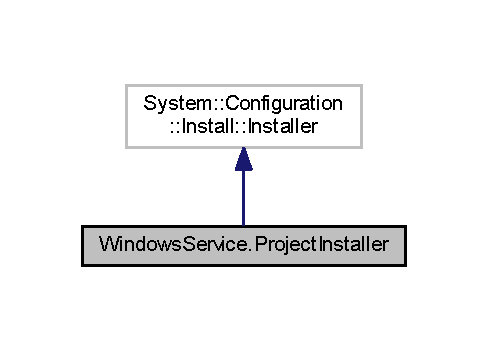
\includegraphics[width=234pt]{class_windows_service_1_1_project_installer__inherit__graph}
\end{center}
\end{figure}


Collaboration diagram for Windows\-Service.\-Project\-Installer\-:\nopagebreak
\begin{figure}[H]
\begin{center}
\leavevmode
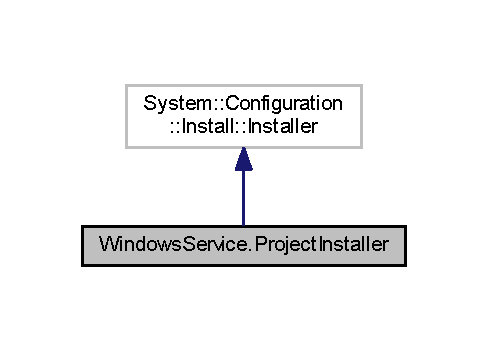
\includegraphics[width=234pt]{class_windows_service_1_1_project_installer__coll__graph}
\end{center}
\end{figure}
\subsection*{Protected Member Functions}
\begin{DoxyCompactItemize}
\item 
override void \hyperlink{class_windows_service_1_1_project_installer_aa57f35eb3d69fcb269363c2bf9445169}{Dispose} (bool disposing)
\begin{DoxyCompactList}\small\item\em Clean up any resources being used. \end{DoxyCompactList}\end{DoxyCompactItemize}


\subsection{Member Function Documentation}
\hypertarget{class_windows_service_1_1_project_installer_aa57f35eb3d69fcb269363c2bf9445169}{\index{Windows\-Service\-::\-Project\-Installer@{Windows\-Service\-::\-Project\-Installer}!Dispose@{Dispose}}
\index{Dispose@{Dispose}!WindowsService::ProjectInstaller@{Windows\-Service\-::\-Project\-Installer}}
\subsubsection[{Dispose}]{\setlength{\rightskip}{0pt plus 5cm}override void Windows\-Service.\-Project\-Installer.\-Dispose (
\begin{DoxyParamCaption}
\item[{bool}]{disposing}
\end{DoxyParamCaption}
)\hspace{0.3cm}{\ttfamily [protected]}}}\label{class_windows_service_1_1_project_installer_aa57f35eb3d69fcb269363c2bf9445169}


Clean up any resources being used. 


\begin{DoxyParams}{Parameters}
{\em disposing} & true if managed resources should be disposed; otherwise, false.\\
\hline
\end{DoxyParams}


The documentation for this class was generated from the following files\-:\begin{DoxyCompactItemize}
\item 
Windows\-Service/Project\-Installer.\-cs\item 
Windows\-Service/Project\-Installer.\-Designer.\-cs\end{DoxyCompactItemize}

\hypertarget{class_service_library_1_1_response}{\section{Service\-Library.\-Response Class Reference}
\label{class_service_library_1_1_response}\index{Service\-Library.\-Response@{Service\-Library.\-Response}}
}


Class to handle response of the rest framework  


\subsection*{Static Public Member Functions}
\begin{DoxyCompactItemize}
\item 
static Stream \hyperlink{class_service_library_1_1_response_a725731173a26e1f6c589d6bd5bea564c}{Serialize} (bool status, int error, object result)
\begin{DoxyCompactList}\small\item\em Serialises the object into json. \end{DoxyCompactList}\end{DoxyCompactItemize}


\subsection{Detailed Description}
Class to handle response of the rest framework 



\subsection{Member Function Documentation}
\hypertarget{class_service_library_1_1_response_a725731173a26e1f6c589d6bd5bea564c}{\index{Service\-Library\-::\-Response@{Service\-Library\-::\-Response}!Serialize@{Serialize}}
\index{Serialize@{Serialize}!ServiceLibrary::Response@{Service\-Library\-::\-Response}}
\subsubsection[{Serialize}]{\setlength{\rightskip}{0pt plus 5cm}static Stream Service\-Library.\-Response.\-Serialize (
\begin{DoxyParamCaption}
\item[{bool}]{status, }
\item[{int}]{error, }
\item[{object}]{result}
\end{DoxyParamCaption}
)\hspace{0.3cm}{\ttfamily [static]}}}\label{class_service_library_1_1_response_a725731173a26e1f6c589d6bd5bea564c}


Serialises the object into json. 


\begin{DoxyParams}{Parameters}
{\em status} & Bool for whether function succeeded\\
\hline
{\em error} & Error code to return\\
\hline
{\em result} & Object for which result is contained\\
\hline
\end{DoxyParams}
\begin{DoxyReturn}{Returns}
Returns memorystream for full control of output data
\end{DoxyReturn}


The documentation for this class was generated from the following file\-:\begin{DoxyCompactItemize}
\item 
Service\-Library/response.\-cs\end{DoxyCompactItemize}

\hypertarget{class_service_library_1_1_database_1_1_rest_entities}{\section{Service\-Library.\-Database.\-Rest\-Entities Class Reference}
\label{class_service_library_1_1_database_1_1_rest_entities}\index{Service\-Library.\-Database.\-Rest\-Entities@{Service\-Library.\-Database.\-Rest\-Entities}}
}


Inheritance diagram for Service\-Library.\-Database.\-Rest\-Entities\-:\nopagebreak
\begin{figure}[H]
\begin{center}
\leavevmode
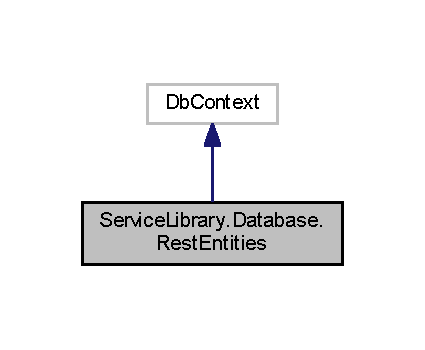
\includegraphics[width=204pt]{class_service_library_1_1_database_1_1_rest_entities__inherit__graph}
\end{center}
\end{figure}


Collaboration diagram for Service\-Library.\-Database.\-Rest\-Entities\-:\nopagebreak
\begin{figure}[H]
\begin{center}
\leavevmode
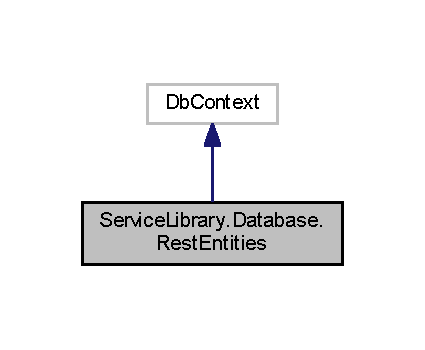
\includegraphics[width=204pt]{class_service_library_1_1_database_1_1_rest_entities__coll__graph}
\end{center}
\end{figure}
\subsection*{Protected Member Functions}
\begin{DoxyCompactItemize}
\item 
\hypertarget{class_service_library_1_1_database_1_1_rest_entities_ae6312489581da4a907f51a692245a2a5}{override void {\bfseries On\-Model\-Creating} (Db\-Model\-Builder model\-Builder)}\label{class_service_library_1_1_database_1_1_rest_entities_ae6312489581da4a907f51a692245a2a5}

\end{DoxyCompactItemize}
\subsection*{Properties}
\begin{DoxyCompactItemize}
\item 
\hypertarget{class_service_library_1_1_database_1_1_rest_entities_a762fe35c778d313557d6b9ffd909ad4d}{Db\-Set$<$ \hyperlink{class_service_library_1_1_database_1_1fleamarket__addresses}{fleamarket\-\_\-addresses} $>$ {\bfseries fleamarket\-\_\-addresses}\hspace{0.3cm}{\ttfamily  \mbox{[}get, set\mbox{]}}}\label{class_service_library_1_1_database_1_1_rest_entities_a762fe35c778d313557d6b9ffd909ad4d}

\item 
\hypertarget{class_service_library_1_1_database_1_1_rest_entities_a9a9f04136afa40bc4189d13e5ca01ffa}{Db\-Set$<$ \hyperlink{class_service_library_1_1_database_1_1fleamarket__items}{fleamarket\-\_\-items} $>$ {\bfseries fleamarket\-\_\-items}\hspace{0.3cm}{\ttfamily  \mbox{[}get, set\mbox{]}}}\label{class_service_library_1_1_database_1_1_rest_entities_a9a9f04136afa40bc4189d13e5ca01ffa}

\item 
\hypertarget{class_service_library_1_1_database_1_1_rest_entities_a7af8a7ff747b687d3a52c2338263e8f7}{Db\-Set$<$ \hyperlink{class_service_library_1_1_database_1_1fleamarket__openings}{fleamarket\-\_\-openings} $>$ {\bfseries fleamarket\-\_\-openings}\hspace{0.3cm}{\ttfamily  \mbox{[}get, set\mbox{]}}}\label{class_service_library_1_1_database_1_1_rest_entities_a7af8a7ff747b687d3a52c2338263e8f7}

\item 
\hypertarget{class_service_library_1_1_database_1_1_rest_entities_aee86d8e6a54e660ee023695055191d46}{Db\-Set$<$ \hyperlink{class_service_library_1_1_database_1_1fleamarket__reviews}{fleamarket\-\_\-reviews} $>$ {\bfseries fleamarket\-\_\-reviews}\hspace{0.3cm}{\ttfamily  \mbox{[}get, set\mbox{]}}}\label{class_service_library_1_1_database_1_1_rest_entities_aee86d8e6a54e660ee023695055191d46}

\item 
\hypertarget{class_service_library_1_1_database_1_1_rest_entities_a8330d574c4ff37347e6a00387ed2c1ae}{Db\-Set$<$ \hyperlink{class_service_library_1_1_database_1_1fleamarkets}{fleamarkets} $>$ {\bfseries fleamarkets}\hspace{0.3cm}{\ttfamily  \mbox{[}get, set\mbox{]}}}\label{class_service_library_1_1_database_1_1_rest_entities_a8330d574c4ff37347e6a00387ed2c1ae}

\item 
\hypertarget{class_service_library_1_1_database_1_1_rest_entities_a00aa8a90a5886f687c500f378e96adb5}{Db\-Set$<$ \hyperlink{class_service_library_1_1_database_1_1users}{users} $>$ {\bfseries users}\hspace{0.3cm}{\ttfamily  \mbox{[}get, set\mbox{]}}}\label{class_service_library_1_1_database_1_1_rest_entities_a00aa8a90a5886f687c500f378e96adb5}

\end{DoxyCompactItemize}


The documentation for this class was generated from the following file\-:\begin{DoxyCompactItemize}
\item 
Service\-Library/\-Database/R\-E\-S\-T.\-Context.\-cs\end{DoxyCompactItemize}

\hypertarget{class_service_library_1_1_rest_service}{\section{Service\-Library.\-Rest\-Service Class Reference}
\label{class_service_library_1_1_rest_service}\index{Service\-Library.\-Rest\-Service@{Service\-Library.\-Rest\-Service}}
}


Inheritance diagram for Service\-Library.\-Rest\-Service\-:\nopagebreak
\begin{figure}[H]
\begin{center}
\leavevmode
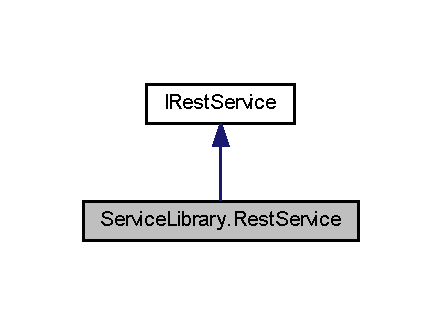
\includegraphics[width=212pt]{class_service_library_1_1_rest_service__inherit__graph}
\end{center}
\end{figure}


Collaboration diagram for Service\-Library.\-Rest\-Service\-:\nopagebreak
\begin{figure}[H]
\begin{center}
\leavevmode
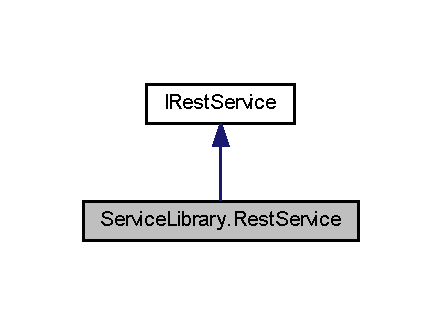
\includegraphics[width=212pt]{class_service_library_1_1_rest_service__coll__graph}
\end{center}
\end{figure}
\subsection*{Public Member Functions}
\begin{DoxyCompactItemize}
\item 
Stream \hyperlink{class_service_library_1_1_rest_service_a5ac245dc76449e578d8f47df0344332a}{fleamarket\-List} ()
\begin{DoxyCompactList}\small\item\em Function that shows all fleamarkets \end{DoxyCompactList}\item 
Stream \hyperlink{class_service_library_1_1_rest_service_aafc5b16ec37b4b2d75d57335fc155650}{fleamarket\-Description} (string id)
\begin{DoxyCompactList}\small\item\em Function that gets info about a specific market \end{DoxyCompactList}\item 
Stream \hyperlink{class_service_library_1_1_rest_service_a099ea56300324e0f53b447469579e363}{register} (string username, string password)
\begin{DoxyCompactList}\small\item\em Function that registers a user with given parameters \end{DoxyCompactList}\item 
Stream \hyperlink{class_service_library_1_1_rest_service_a31577832960f1aaf0c93f81e5134272a}{login} (string username, string password)
\begin{DoxyCompactList}\small\item\em Function that checks if a username/password is a valid user \end{DoxyCompactList}\item 
Stream \hyperlink{class_service_library_1_1_rest_service_a0121954034b57e8947b9c5ce65479f65}{create\-Review} (string username, string password, string fleamarket\-Id, string stars, string text)
\begin{DoxyCompactList}\small\item\em Function to create review of a fleamarket, if authorised \end{DoxyCompactList}\item 
Stream \hyperlink{class_service_library_1_1_rest_service_a7623f407a00d3bc2f93b12168c7674b5}{update\-Review} (string username, string password, string fleamarket\-Id, string stars, string text)
\begin{DoxyCompactList}\small\item\em Function to update an existing review if authorised \end{DoxyCompactList}\item 
Stream \hyperlink{class_service_library_1_1_rest_service_ad0b87d313f13ec52372edafd6cac9c09}{delete\-Review} (string username, string password, string fleamarket\-Id)
\begin{DoxyCompactList}\small\item\em Function to delete existing reviews if authorised \end{DoxyCompactList}\item 
Stream \hyperlink{class_service_library_1_1_rest_service_a39a86dadc6525bee03594f583acff2da}{create\-Flea\-Market} (string username, string password, string name, string description, string logo, string category, string city, string street, string postcode, string latitude, string longitude)
\begin{DoxyCompactList}\small\item\em Creates a fleamarket on the database if authorised for it \end{DoxyCompactList}\item 
Stream \hyperlink{class_service_library_1_1_rest_service_a3e183c1c796a74337fdfac3070036066}{update\-Flea\-Market} (string username, string password, string fleamarket\-Id, string name, string description, string logo, string category, string city, string street, string postcode, string latitude, string longitude)
\begin{DoxyCompactList}\small\item\em Updates a certain fleamarket if authorised for it \end{DoxyCompactList}\item 
Stream \hyperlink{class_service_library_1_1_rest_service_ab502a53d2f520a2b43803a10cb8a93d2}{delete\-Flea\-Market} (string username, string password, string fleamarket\-Id)
\begin{DoxyCompactList}\small\item\em Function that deletes a certain fleamarket if authorised for it \end{DoxyCompactList}\item 
Stream \hyperlink{class_service_library_1_1_rest_service_a4d3293e03679b4d959f342308da43b1f}{create\-Opening} (string username, string password, string fleamarket\-Id, string from, string to, string description)
\begin{DoxyCompactList}\small\item\em Function that creates fleamarket openings if authorised for it \end{DoxyCompactList}\item 
Stream \hyperlink{class_service_library_1_1_rest_service_a1fb0b2b9aabae6add481c8599579044a}{update\-Opening} (string username, string password, string opening\-Id, string from, string to, string description)
\begin{DoxyCompactList}\small\item\em Function that updates an existing opening if authorised for it \end{DoxyCompactList}\item 
Stream \hyperlink{class_service_library_1_1_rest_service_a7952a882cc96c062c8ac5ddaaf56030f}{delete\-Opening} (string username, string password, string opening\-Id)
\begin{DoxyCompactList}\small\item\em Function that deletes an existing opening if authorised for it \end{DoxyCompactList}\end{DoxyCompactItemize}


\subsection{Member Function Documentation}
\hypertarget{class_service_library_1_1_rest_service_a39a86dadc6525bee03594f583acff2da}{\index{Service\-Library\-::\-Rest\-Service@{Service\-Library\-::\-Rest\-Service}!create\-Flea\-Market@{create\-Flea\-Market}}
\index{create\-Flea\-Market@{create\-Flea\-Market}!ServiceLibrary::RestService@{Service\-Library\-::\-Rest\-Service}}
\subsubsection[{create\-Flea\-Market}]{\setlength{\rightskip}{0pt plus 5cm}Stream Service\-Library.\-Rest\-Service.\-create\-Flea\-Market (
\begin{DoxyParamCaption}
\item[{string}]{username, }
\item[{string}]{password, }
\item[{string}]{name, }
\item[{string}]{description, }
\item[{string}]{logo, }
\item[{string}]{category, }
\item[{string}]{city, }
\item[{string}]{street, }
\item[{string}]{postcode, }
\item[{string}]{latitude, }
\item[{string}]{longitude}
\end{DoxyParamCaption}
)}}\label{class_service_library_1_1_rest_service_a39a86dadc6525bee03594f583acff2da}


Creates a fleamarket on the database if authorised for it 


\begin{DoxyParams}{Parameters}
{\em username} & Username of the user that wanna add market\\
\hline
{\em password} & Password of the user that wanna add market\\
\hline
{\em name} & Name of the fleamarket\\
\hline
{\em description} & Description of the fleamarket\\
\hline
{\em logo} & Logo of the fleamarket\\
\hline
{\em category} & Category of the fleamarket\\
\hline
{\em city} & City of the fleamarket\\
\hline
{\em street} & Street of the fleamarket\\
\hline
{\em postcode} & Postcode of the fleamarket\\
\hline
{\em latitude} & Latitude of the fleamarket\\
\hline
{\em longitude} & Longitude of the fleamarket\\
\hline
\end{DoxyParams}
\begin{DoxyReturn}{Returns}
J\-S\-O\-N of a wrapper with status
\end{DoxyReturn}


Implements \hyperlink{interface_service_library_1_1_i_rest_service_a54317be38e33419acaba46e8ba6a0958}{Service\-Library.\-I\-Rest\-Service}.

\hypertarget{class_service_library_1_1_rest_service_a4d3293e03679b4d959f342308da43b1f}{\index{Service\-Library\-::\-Rest\-Service@{Service\-Library\-::\-Rest\-Service}!create\-Opening@{create\-Opening}}
\index{create\-Opening@{create\-Opening}!ServiceLibrary::RestService@{Service\-Library\-::\-Rest\-Service}}
\subsubsection[{create\-Opening}]{\setlength{\rightskip}{0pt plus 5cm}Stream Service\-Library.\-Rest\-Service.\-create\-Opening (
\begin{DoxyParamCaption}
\item[{string}]{username, }
\item[{string}]{password, }
\item[{string}]{fleamarket\-Id, }
\item[{string}]{from, }
\item[{string}]{to, }
\item[{string}]{description}
\end{DoxyParamCaption}
)}}\label{class_service_library_1_1_rest_service_a4d3293e03679b4d959f342308da43b1f}


Function that creates fleamarket openings if authorised for it 


\begin{DoxyParams}{Parameters}
{\em username} & Username of the user wanting to add opening\\
\hline
{\em password} & Password of the user wanting to add opening\\
\hline
{\em fleamarket\-Id} & Id of the fleamarket to add opening\\
\hline
{\em from} & Datetime of the from time\\
\hline
{\em to} & Datetime of the to time\\
\hline
{\em description} & Description of the time\\
\hline
\end{DoxyParams}
\begin{DoxyReturn}{Returns}
J\-S\-O\-N of a wrapper with status
\end{DoxyReturn}


Implements \hyperlink{interface_service_library_1_1_i_rest_service_a8da12dfeb7d26f50c935c17ed4969ef8}{Service\-Library.\-I\-Rest\-Service}.

\hypertarget{class_service_library_1_1_rest_service_a0121954034b57e8947b9c5ce65479f65}{\index{Service\-Library\-::\-Rest\-Service@{Service\-Library\-::\-Rest\-Service}!create\-Review@{create\-Review}}
\index{create\-Review@{create\-Review}!ServiceLibrary::RestService@{Service\-Library\-::\-Rest\-Service}}
\subsubsection[{create\-Review}]{\setlength{\rightskip}{0pt plus 5cm}Stream Service\-Library.\-Rest\-Service.\-create\-Review (
\begin{DoxyParamCaption}
\item[{string}]{username, }
\item[{string}]{password, }
\item[{string}]{fleamarket\-Id, }
\item[{string}]{stars, }
\item[{string}]{text}
\end{DoxyParamCaption}
)}}\label{class_service_library_1_1_rest_service_a0121954034b57e8947b9c5ce65479f65}


Function to create review of a fleamarket, if authorised 


\begin{DoxyParams}{Parameters}
{\em username} & Username of the user wanting to create review\\
\hline
{\em password} & Password of the user wanting to create review\\
\hline
{\em fleamarket\-Id} & Id of fleamarket to add review\\
\hline
{\em stars} & Amount of stars for review\\
\hline
{\em text} & Text for the review\\
\hline
\end{DoxyParams}
\begin{DoxyReturn}{Returns}
J\-S\-O\-N of a wrapper with status
\end{DoxyReturn}


Implements \hyperlink{interface_service_library_1_1_i_rest_service_a925656ba45a706648af391a00733e45f}{Service\-Library.\-I\-Rest\-Service}.

\hypertarget{class_service_library_1_1_rest_service_ab502a53d2f520a2b43803a10cb8a93d2}{\index{Service\-Library\-::\-Rest\-Service@{Service\-Library\-::\-Rest\-Service}!delete\-Flea\-Market@{delete\-Flea\-Market}}
\index{delete\-Flea\-Market@{delete\-Flea\-Market}!ServiceLibrary::RestService@{Service\-Library\-::\-Rest\-Service}}
\subsubsection[{delete\-Flea\-Market}]{\setlength{\rightskip}{0pt plus 5cm}Stream Service\-Library.\-Rest\-Service.\-delete\-Flea\-Market (
\begin{DoxyParamCaption}
\item[{string}]{username, }
\item[{string}]{password, }
\item[{string}]{fleamarket\-Id}
\end{DoxyParamCaption}
)}}\label{class_service_library_1_1_rest_service_ab502a53d2f520a2b43803a10cb8a93d2}


Function that deletes a certain fleamarket if authorised for it 


\begin{DoxyParams}{Parameters}
{\em username} & Username of the user wanting to delete a market\\
\hline
{\em password} & Password of the user wanting to delete a market\\
\hline
{\em fleamarket\-Id} & Id of the market to be deleted\\
\hline
\end{DoxyParams}
\begin{DoxyReturn}{Returns}
J\-S\-O\-N of a wrapper with status
\end{DoxyReturn}


Implements \hyperlink{interface_service_library_1_1_i_rest_service_ab1f44acad37127065148c804d03fc36f}{Service\-Library.\-I\-Rest\-Service}.

\hypertarget{class_service_library_1_1_rest_service_a7952a882cc96c062c8ac5ddaaf56030f}{\index{Service\-Library\-::\-Rest\-Service@{Service\-Library\-::\-Rest\-Service}!delete\-Opening@{delete\-Opening}}
\index{delete\-Opening@{delete\-Opening}!ServiceLibrary::RestService@{Service\-Library\-::\-Rest\-Service}}
\subsubsection[{delete\-Opening}]{\setlength{\rightskip}{0pt plus 5cm}Stream Service\-Library.\-Rest\-Service.\-delete\-Opening (
\begin{DoxyParamCaption}
\item[{string}]{username, }
\item[{string}]{password, }
\item[{string}]{opening\-Id}
\end{DoxyParamCaption}
)}}\label{class_service_library_1_1_rest_service_a7952a882cc96c062c8ac5ddaaf56030f}


Function that deletes an existing opening if authorised for it 


\begin{DoxyParams}{Parameters}
{\em username} & Username of the user wanting to delete opening\\
\hline
{\em password} & Password of the user wanting to delete opening\\
\hline
{\em opening\-Id} & Id of opening to be deleted\\
\hline
\end{DoxyParams}
\begin{DoxyReturn}{Returns}
J\-S\-O\-N of a wrapper with status
\end{DoxyReturn}


Implements \hyperlink{interface_service_library_1_1_i_rest_service_a4bfa508142405715bb37792073c43eb2}{Service\-Library.\-I\-Rest\-Service}.

\hypertarget{class_service_library_1_1_rest_service_ad0b87d313f13ec52372edafd6cac9c09}{\index{Service\-Library\-::\-Rest\-Service@{Service\-Library\-::\-Rest\-Service}!delete\-Review@{delete\-Review}}
\index{delete\-Review@{delete\-Review}!ServiceLibrary::RestService@{Service\-Library\-::\-Rest\-Service}}
\subsubsection[{delete\-Review}]{\setlength{\rightskip}{0pt plus 5cm}Stream Service\-Library.\-Rest\-Service.\-delete\-Review (
\begin{DoxyParamCaption}
\item[{string}]{username, }
\item[{string}]{password, }
\item[{string}]{fleamarket\-Id}
\end{DoxyParamCaption}
)}}\label{class_service_library_1_1_rest_service_ad0b87d313f13ec52372edafd6cac9c09}


Function to delete existing reviews if authorised 


\begin{DoxyParams}{Parameters}
{\em username} & Username of the user wanting to delete review\\
\hline
{\em password} & Password of the user wanting to delete review\\
\hline
{\em fleamarket\-Id} & Id of fleamarket to delete review from\\
\hline
\end{DoxyParams}
\begin{DoxyReturn}{Returns}
J\-S\-O\-N of a wrapper with status
\end{DoxyReturn}


Implements \hyperlink{interface_service_library_1_1_i_rest_service_ae8340be9ca2f22dc5e3e93e7d2786c85}{Service\-Library.\-I\-Rest\-Service}.

\hypertarget{class_service_library_1_1_rest_service_aafc5b16ec37b4b2d75d57335fc155650}{\index{Service\-Library\-::\-Rest\-Service@{Service\-Library\-::\-Rest\-Service}!fleamarket\-Description@{fleamarket\-Description}}
\index{fleamarket\-Description@{fleamarket\-Description}!ServiceLibrary::RestService@{Service\-Library\-::\-Rest\-Service}}
\subsubsection[{fleamarket\-Description}]{\setlength{\rightskip}{0pt plus 5cm}Stream Service\-Library.\-Rest\-Service.\-fleamarket\-Description (
\begin{DoxyParamCaption}
\item[{string}]{id}
\end{DoxyParamCaption}
)}}\label{class_service_library_1_1_rest_service_aafc5b16ec37b4b2d75d57335fc155650}


Function that gets info about a specific market 


\begin{DoxyParams}{Parameters}
{\em id} & Id of the market to get details about\\
\hline
\end{DoxyParams}
\begin{DoxyReturn}{Returns}
J\-S\-O\-N of a wrapper with details of a specific market
\end{DoxyReturn}


Implements \hyperlink{interface_service_library_1_1_i_rest_service_af1be4751f78a02a57e702a69054632cc}{Service\-Library.\-I\-Rest\-Service}.

\hypertarget{class_service_library_1_1_rest_service_a5ac245dc76449e578d8f47df0344332a}{\index{Service\-Library\-::\-Rest\-Service@{Service\-Library\-::\-Rest\-Service}!fleamarket\-List@{fleamarket\-List}}
\index{fleamarket\-List@{fleamarket\-List}!ServiceLibrary::RestService@{Service\-Library\-::\-Rest\-Service}}
\subsubsection[{fleamarket\-List}]{\setlength{\rightskip}{0pt plus 5cm}Stream Service\-Library.\-Rest\-Service.\-fleamarket\-List (
\begin{DoxyParamCaption}
{}
\end{DoxyParamCaption}
)}}\label{class_service_library_1_1_rest_service_a5ac245dc76449e578d8f47df0344332a}


Function that shows all fleamarkets 

\begin{DoxyReturn}{Returns}
J\-S\-O\-N of a wrapper with all fleamarkets
\end{DoxyReturn}


Implements \hyperlink{interface_service_library_1_1_i_rest_service_ad6d9e2dcc4d575310586390fa144d181}{Service\-Library.\-I\-Rest\-Service}.

\hypertarget{class_service_library_1_1_rest_service_a31577832960f1aaf0c93f81e5134272a}{\index{Service\-Library\-::\-Rest\-Service@{Service\-Library\-::\-Rest\-Service}!login@{login}}
\index{login@{login}!ServiceLibrary::RestService@{Service\-Library\-::\-Rest\-Service}}
\subsubsection[{login}]{\setlength{\rightskip}{0pt plus 5cm}Stream Service\-Library.\-Rest\-Service.\-login (
\begin{DoxyParamCaption}
\item[{string}]{username, }
\item[{string}]{password}
\end{DoxyParamCaption}
)}}\label{class_service_library_1_1_rest_service_a31577832960f1aaf0c93f81e5134272a}


Function that checks if a username/password is a valid user 


\begin{DoxyParams}{Parameters}
{\em username} & Username of the user wanting to log in\\
\hline
{\em password} & Password of the user wanting to log in\\
\hline
\end{DoxyParams}
\begin{DoxyReturn}{Returns}
J\-S\-O\-N of a wrapper with status
\end{DoxyReturn}


Implements \hyperlink{interface_service_library_1_1_i_rest_service_aa0ee715b0c69f4c024ede0d91939c4a2}{Service\-Library.\-I\-Rest\-Service}.

\hypertarget{class_service_library_1_1_rest_service_a099ea56300324e0f53b447469579e363}{\index{Service\-Library\-::\-Rest\-Service@{Service\-Library\-::\-Rest\-Service}!register@{register}}
\index{register@{register}!ServiceLibrary::RestService@{Service\-Library\-::\-Rest\-Service}}
\subsubsection[{register}]{\setlength{\rightskip}{0pt plus 5cm}Stream Service\-Library.\-Rest\-Service.\-register (
\begin{DoxyParamCaption}
\item[{string}]{username, }
\item[{string}]{password}
\end{DoxyParamCaption}
)}}\label{class_service_library_1_1_rest_service_a099ea56300324e0f53b447469579e363}


Function that registers a user with given parameters 


\begin{DoxyParams}{Parameters}
{\em username} & Username the user wants\\
\hline
{\em password} & Password the user wants\\
\hline
\end{DoxyParams}
\begin{DoxyReturn}{Returns}
J\-S\-O\-N of a wrapper with status
\end{DoxyReturn}


Implements \hyperlink{interface_service_library_1_1_i_rest_service_ae566a85d019d87c013ed069b381e59ee}{Service\-Library.\-I\-Rest\-Service}.

\hypertarget{class_service_library_1_1_rest_service_a3e183c1c796a74337fdfac3070036066}{\index{Service\-Library\-::\-Rest\-Service@{Service\-Library\-::\-Rest\-Service}!update\-Flea\-Market@{update\-Flea\-Market}}
\index{update\-Flea\-Market@{update\-Flea\-Market}!ServiceLibrary::RestService@{Service\-Library\-::\-Rest\-Service}}
\subsubsection[{update\-Flea\-Market}]{\setlength{\rightskip}{0pt plus 5cm}Stream Service\-Library.\-Rest\-Service.\-update\-Flea\-Market (
\begin{DoxyParamCaption}
\item[{string}]{username, }
\item[{string}]{password, }
\item[{string}]{fleamarket\-Id, }
\item[{string}]{name, }
\item[{string}]{description, }
\item[{string}]{logo, }
\item[{string}]{category, }
\item[{string}]{city, }
\item[{string}]{street, }
\item[{string}]{postcode, }
\item[{string}]{latitude, }
\item[{string}]{longitude}
\end{DoxyParamCaption}
)}}\label{class_service_library_1_1_rest_service_a3e183c1c796a74337fdfac3070036066}


Updates a certain fleamarket if authorised for it 


\begin{DoxyParams}{Parameters}
{\em username} & Username of the user that wanna update market\\
\hline
{\em password} & Password of the user that wanna update market\\
\hline
{\em fleamarket\-Id} & Fleamarket id of the market to update\\
\hline
{\em name} & Name of which to change fleamarket to\\
\hline
{\em description} & Description of which to change fleamarket to\\
\hline
{\em logo} & Logo of which to change fleamarket to\\
\hline
{\em category} & Category of which to change fleamarket to\\
\hline
{\em city} & City of which to change fleamarket to\\
\hline
{\em street} & Street of which to change fleamarket to\\
\hline
{\em postcode} & Postcode of which to change fleamarket to\\
\hline
{\em latitude} & Latitude of which to change fleamarket to\\
\hline
{\em longitude} & Longitude of which to change fleamarket to\\
\hline
\end{DoxyParams}
\begin{DoxyReturn}{Returns}
J\-S\-O\-N of a wrapper with status
\end{DoxyReturn}


Implements \hyperlink{interface_service_library_1_1_i_rest_service_a6a7bcc09960ff24c5ce779e7be7d4ddb}{Service\-Library.\-I\-Rest\-Service}.

\hypertarget{class_service_library_1_1_rest_service_a1fb0b2b9aabae6add481c8599579044a}{\index{Service\-Library\-::\-Rest\-Service@{Service\-Library\-::\-Rest\-Service}!update\-Opening@{update\-Opening}}
\index{update\-Opening@{update\-Opening}!ServiceLibrary::RestService@{Service\-Library\-::\-Rest\-Service}}
\subsubsection[{update\-Opening}]{\setlength{\rightskip}{0pt plus 5cm}Stream Service\-Library.\-Rest\-Service.\-update\-Opening (
\begin{DoxyParamCaption}
\item[{string}]{username, }
\item[{string}]{password, }
\item[{string}]{opening\-Id, }
\item[{string}]{from, }
\item[{string}]{to, }
\item[{string}]{description}
\end{DoxyParamCaption}
)}}\label{class_service_library_1_1_rest_service_a1fb0b2b9aabae6add481c8599579044a}


Function that updates an existing opening if authorised for it 


\begin{DoxyParams}{Parameters}
{\em username} & Username of the user wanting to edit opening\\
\hline
{\em password} & Password of the user wanting to edit opening\\
\hline
{\em opening\-Id} & Id of the opening to be updated\\
\hline
{\em from} & Datetime of from time\\
\hline
{\em to} & Datetime of to time\\
\hline
{\em description} & Description of the time\\
\hline
\end{DoxyParams}
\begin{DoxyReturn}{Returns}
J\-S\-O\-N of a wrapper with status
\end{DoxyReturn}


Implements \hyperlink{interface_service_library_1_1_i_rest_service_aff55a9fbcda58a0830319982233420b8}{Service\-Library.\-I\-Rest\-Service}.

\hypertarget{class_service_library_1_1_rest_service_a7623f407a00d3bc2f93b12168c7674b5}{\index{Service\-Library\-::\-Rest\-Service@{Service\-Library\-::\-Rest\-Service}!update\-Review@{update\-Review}}
\index{update\-Review@{update\-Review}!ServiceLibrary::RestService@{Service\-Library\-::\-Rest\-Service}}
\subsubsection[{update\-Review}]{\setlength{\rightskip}{0pt plus 5cm}Stream Service\-Library.\-Rest\-Service.\-update\-Review (
\begin{DoxyParamCaption}
\item[{string}]{username, }
\item[{string}]{password, }
\item[{string}]{fleamarket\-Id, }
\item[{string}]{stars, }
\item[{string}]{text}
\end{DoxyParamCaption}
)}}\label{class_service_library_1_1_rest_service_a7623f407a00d3bc2f93b12168c7674b5}


Function to update an existing review if authorised 


\begin{DoxyParams}{Parameters}
{\em username} & Username of the user updating review\\
\hline
{\em password} & Password of the user updating review\\
\hline
{\em fleamarket\-Id} & Fleamarket id for which to change review on\\
\hline
{\em stars} & Amount of stars for review change\\
\hline
{\em text} & Text for which to change on review\\
\hline
\end{DoxyParams}
\begin{DoxyReturn}{Returns}
J\-S\-O\-N of a wrapper with status
\end{DoxyReturn}


Implements \hyperlink{interface_service_library_1_1_i_rest_service_a8d80e4dac07cf691bc685c1944192f22}{Service\-Library.\-I\-Rest\-Service}.



The documentation for this class was generated from the following file\-:\begin{DoxyCompactItemize}
\item 
Service\-Library/Rest\-Service.\-cs\end{DoxyCompactItemize}

\hypertarget{class_windows_service_1_1_service}{\section{Windows\-Service.\-Service Class Reference}
\label{class_windows_service_1_1_service}\index{Windows\-Service.\-Service@{Windows\-Service.\-Service}}
}


Inheritance diagram for Windows\-Service.\-Service\-:\nopagebreak
\begin{figure}[H]
\begin{center}
\leavevmode
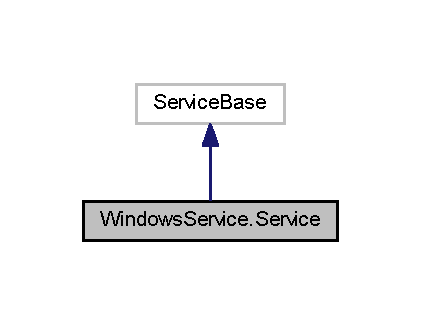
\includegraphics[width=202pt]{class_windows_service_1_1_service__inherit__graph}
\end{center}
\end{figure}


Collaboration diagram for Windows\-Service.\-Service\-:\nopagebreak
\begin{figure}[H]
\begin{center}
\leavevmode
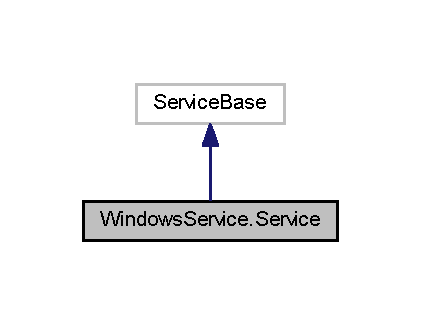
\includegraphics[width=202pt]{class_windows_service_1_1_service__coll__graph}
\end{center}
\end{figure}
\subsection*{Protected Member Functions}
\begin{DoxyCompactItemize}
\item 
\hypertarget{class_windows_service_1_1_service_aab88ecc6da7cc097db05fa7da846c659}{override void {\bfseries On\-Start} (string\mbox{[}$\,$\mbox{]} args)}\label{class_windows_service_1_1_service_aab88ecc6da7cc097db05fa7da846c659}

\item 
\hypertarget{class_windows_service_1_1_service_a899e4fd379d76037b4b73532b9d11477}{override void {\bfseries On\-Stop} ()}\label{class_windows_service_1_1_service_a899e4fd379d76037b4b73532b9d11477}

\item 
override void \hyperlink{class_windows_service_1_1_service_acc90068d55c4f0ea2ab64eb66ebfff31}{Dispose} (bool disposing)
\begin{DoxyCompactList}\small\item\em Clean up any resources being used. \end{DoxyCompactList}\end{DoxyCompactItemize}


\subsection{Member Function Documentation}
\hypertarget{class_windows_service_1_1_service_acc90068d55c4f0ea2ab64eb66ebfff31}{\index{Windows\-Service\-::\-Service@{Windows\-Service\-::\-Service}!Dispose@{Dispose}}
\index{Dispose@{Dispose}!WindowsService::Service@{Windows\-Service\-::\-Service}}
\subsubsection[{Dispose}]{\setlength{\rightskip}{0pt plus 5cm}override void Windows\-Service.\-Service.\-Dispose (
\begin{DoxyParamCaption}
\item[{bool}]{disposing}
\end{DoxyParamCaption}
)\hspace{0.3cm}{\ttfamily [protected]}}}\label{class_windows_service_1_1_service_acc90068d55c4f0ea2ab64eb66ebfff31}


Clean up any resources being used. 


\begin{DoxyParams}{Parameters}
{\em disposing} & true if managed resources should be disposed; otherwise, false.\\
\hline
\end{DoxyParams}


The documentation for this class was generated from the following files\-:\begin{DoxyCompactItemize}
\item 
Windows\-Service/Service.\-cs\item 
Windows\-Service/Service.\-Designer.\-cs\end{DoxyCompactItemize}

\hypertarget{class_service_library_1_1_database_1_1users}{\section{Service\-Library.\-Database.\-users Class Reference}
\label{class_service_library_1_1_database_1_1users}\index{Service\-Library.\-Database.\-users@{Service\-Library.\-Database.\-users}}
}
\subsection*{Properties}
\begin{DoxyCompactItemize}
\item 
\hypertarget{class_service_library_1_1_database_1_1users_a10c9c0bc565ccb97257775501160e535}{int {\bfseries id}\hspace{0.3cm}{\ttfamily  \mbox{[}get, set\mbox{]}}}\label{class_service_library_1_1_database_1_1users_a10c9c0bc565ccb97257775501160e535}

\item 
\hypertarget{class_service_library_1_1_database_1_1users_a00e3e41e170b4fe7b655a6069ae163a1}{string {\bfseries email}\hspace{0.3cm}{\ttfamily  \mbox{[}get, set\mbox{]}}}\label{class_service_library_1_1_database_1_1users_a00e3e41e170b4fe7b655a6069ae163a1}

\item 
\hypertarget{class_service_library_1_1_database_1_1users_a8f9efd15895a9e0e9f981697259786f3}{string {\bfseries name}\hspace{0.3cm}{\ttfamily  \mbox{[}get, set\mbox{]}}}\label{class_service_library_1_1_database_1_1users_a8f9efd15895a9e0e9f981697259786f3}

\item 
\hypertarget{class_service_library_1_1_database_1_1users_aa63a319d0addf66430a084632853f07a}{string {\bfseries password\-\_\-hash}\hspace{0.3cm}{\ttfamily  \mbox{[}get, set\mbox{]}}}\label{class_service_library_1_1_database_1_1users_aa63a319d0addf66430a084632853f07a}

\item 
\hypertarget{class_service_library_1_1_database_1_1users_ac37d4eefac4cf9977c0d7691e6b67640}{string {\bfseries salt}\hspace{0.3cm}{\ttfamily  \mbox{[}get, set\mbox{]}}}\label{class_service_library_1_1_database_1_1users_ac37d4eefac4cf9977c0d7691e6b67640}

\item 
\hypertarget{class_service_library_1_1_database_1_1users_a815b727479c302618e38348e1ae7afa9}{System.\-Date\-Time {\bfseries created\-\_\-on}\hspace{0.3cm}{\ttfamily  \mbox{[}get, set\mbox{]}}}\label{class_service_library_1_1_database_1_1users_a815b727479c302618e38348e1ae7afa9}

\item 
\hypertarget{class_service_library_1_1_database_1_1users_af5f80d334bb21d5b3bf105ab3a82e24d}{System.\-Date\-Time {\bfseries modified\-\_\-on}\hspace{0.3cm}{\ttfamily  \mbox{[}get, set\mbox{]}}}\label{class_service_library_1_1_database_1_1users_af5f80d334bb21d5b3bf105ab3a82e24d}

\item 
\hypertarget{class_service_library_1_1_database_1_1users_add4e06595ab643210dfc180f00007d61}{virtual I\-Collection\\*
$<$ \hyperlink{class_service_library_1_1_database_1_1fleamarket__reviews}{fleamarket\-\_\-reviews} $>$ {\bfseries fleamarket\-\_\-reviews}\hspace{0.3cm}{\ttfamily  \mbox{[}get, set\mbox{]}}}\label{class_service_library_1_1_database_1_1users_add4e06595ab643210dfc180f00007d61}

\item 
\hypertarget{class_service_library_1_1_database_1_1users_a25f7b4d369a3f19d2bc8b33f51865d3b}{virtual I\-Collection$<$ \hyperlink{class_service_library_1_1_database_1_1fleamarkets}{fleamarkets} $>$ {\bfseries fleamarkets}\hspace{0.3cm}{\ttfamily  \mbox{[}get, set\mbox{]}}}\label{class_service_library_1_1_database_1_1users_a25f7b4d369a3f19d2bc8b33f51865d3b}

\end{DoxyCompactItemize}


The documentation for this class was generated from the following file\-:\begin{DoxyCompactItemize}
\item 
Service\-Library/\-Database/users.\-cs\end{DoxyCompactItemize}

\hypertarget{class_service_library_1_1_utility}{\section{Service\-Library.\-Utility Class Reference}
\label{class_service_library_1_1_utility}\index{Service\-Library.\-Utility@{Service\-Library.\-Utility}}
}


\hyperlink{class_service_library_1_1_utility}{Utility} class that serves functions that doesnt belong anywhere specific.  


\subsection*{Public Types}
\begin{DoxyCompactItemize}
\item 
enum \hyperlink{class_service_library_1_1_utility_ab80e4b5079a093a61aa3b7e85e90f751}{Fleamarket\-Category} \{ {\bfseries flea}, 
{\bfseries charity}, 
{\bfseries trunk}, 
{\bfseries other}
 \}
\begin{DoxyCompactList}\small\item\em Containing enum from database \end{DoxyCompactList}\end{DoxyCompactItemize}
\subsection*{Static Public Member Functions}
\begin{DoxyCompactItemize}
\item 
static \hyperlink{class_service_library_1_1_wrapper}{Wrapper} \hyperlink{class_service_library_1_1_utility_aa17bea205486313547850b080f5cea9d}{review\-Validate\-Rules} (string fleamarketid, string stars, string text)
\begin{DoxyCompactList}\small\item\em Function that checks all parameters for a review \end{DoxyCompactList}\item 
static \hyperlink{class_service_library_1_1_wrapper}{Wrapper} \hyperlink{class_service_library_1_1_utility_a11e42ae7e0eabb70fdd87b64c687b2c4}{opening\-Validate\-Rules} (string from, string to, string description)
\begin{DoxyCompactList}\small\item\em Function that parses and checks opening parameters \end{DoxyCompactList}\item 
static \hyperlink{class_service_library_1_1_wrapper}{Wrapper} \hyperlink{class_service_library_1_1_utility_a4f91936b2528e48313886c219294275a}{fleamarket\-Validate\-Rules} (string name, string description, string logo, string category, string city, string street, string postcode, string latitude, string longitude)
\begin{DoxyCompactList}\small\item\em Function that checks parameters for a fleamarket and parses them \end{DoxyCompactList}\end{DoxyCompactItemize}


\subsection{Detailed Description}
\hyperlink{class_service_library_1_1_utility}{Utility} class that serves functions that doesnt belong anywhere specific. 



\subsection{Member Enumeration Documentation}
\hypertarget{class_service_library_1_1_utility_ab80e4b5079a093a61aa3b7e85e90f751}{\index{Service\-Library\-::\-Utility@{Service\-Library\-::\-Utility}!Fleamarket\-Category@{Fleamarket\-Category}}
\index{Fleamarket\-Category@{Fleamarket\-Category}!ServiceLibrary::Utility@{Service\-Library\-::\-Utility}}
\subsubsection[{Fleamarket\-Category}]{\setlength{\rightskip}{0pt plus 5cm}enum {\bf Service\-Library.\-Utility.\-Fleamarket\-Category}}}\label{class_service_library_1_1_utility_ab80e4b5079a093a61aa3b7e85e90f751}


Containing enum from database 



\subsection{Member Function Documentation}
\hypertarget{class_service_library_1_1_utility_a4f91936b2528e48313886c219294275a}{\index{Service\-Library\-::\-Utility@{Service\-Library\-::\-Utility}!fleamarket\-Validate\-Rules@{fleamarket\-Validate\-Rules}}
\index{fleamarket\-Validate\-Rules@{fleamarket\-Validate\-Rules}!ServiceLibrary::Utility@{Service\-Library\-::\-Utility}}
\subsubsection[{fleamarket\-Validate\-Rules}]{\setlength{\rightskip}{0pt plus 5cm}static {\bf Wrapper} Service\-Library.\-Utility.\-fleamarket\-Validate\-Rules (
\begin{DoxyParamCaption}
\item[{string}]{name, }
\item[{string}]{description, }
\item[{string}]{logo, }
\item[{string}]{category, }
\item[{string}]{city, }
\item[{string}]{street, }
\item[{string}]{postcode, }
\item[{string}]{latitude, }
\item[{string}]{longitude}
\end{DoxyParamCaption}
)\hspace{0.3cm}{\ttfamily [static]}}}\label{class_service_library_1_1_utility_a4f91936b2528e48313886c219294275a}


Function that checks parameters for a fleamarket and parses them 


\begin{DoxyParams}{Parameters}
{\em name} & Name of the fleamarket\\
\hline
{\em description} & Description of the fleamarket\\
\hline
{\em logo} & Logo of the fleamarket\\
\hline
{\em category} & Category of the fleamarket\\
\hline
{\em city} & City of the fleamarket\\
\hline
{\em street} & Street of the fleamarket\\
\hline
{\em postcode} & Postcode of the fleamarket\\
\hline
{\em latitude} & Latitude of the fleamarket\\
\hline
{\em longitude} & Longitude of the fleamarket\\
\hline
\end{DoxyParams}
\begin{DoxyReturn}{Returns}
Return wrapper with a fleamarket and address object to take info out of
\end{DoxyReturn}
\hypertarget{class_service_library_1_1_utility_a11e42ae7e0eabb70fdd87b64c687b2c4}{\index{Service\-Library\-::\-Utility@{Service\-Library\-::\-Utility}!opening\-Validate\-Rules@{opening\-Validate\-Rules}}
\index{opening\-Validate\-Rules@{opening\-Validate\-Rules}!ServiceLibrary::Utility@{Service\-Library\-::\-Utility}}
\subsubsection[{opening\-Validate\-Rules}]{\setlength{\rightskip}{0pt plus 5cm}static {\bf Wrapper} Service\-Library.\-Utility.\-opening\-Validate\-Rules (
\begin{DoxyParamCaption}
\item[{string}]{from, }
\item[{string}]{to, }
\item[{string}]{description}
\end{DoxyParamCaption}
)\hspace{0.3cm}{\ttfamily [static]}}}\label{class_service_library_1_1_utility_a11e42ae7e0eabb70fdd87b64c687b2c4}


Function that parses and checks opening parameters 


\begin{DoxyParams}{Parameters}
{\em from} & Datetime representing from\\
\hline
{\em to} & Datetime representing to\\
\hline
{\em description} & Description for opening\\
\hline
\end{DoxyParams}
\begin{DoxyReturn}{Returns}

\end{DoxyReturn}
\hypertarget{class_service_library_1_1_utility_aa17bea205486313547850b080f5cea9d}{\index{Service\-Library\-::\-Utility@{Service\-Library\-::\-Utility}!review\-Validate\-Rules@{review\-Validate\-Rules}}
\index{review\-Validate\-Rules@{review\-Validate\-Rules}!ServiceLibrary::Utility@{Service\-Library\-::\-Utility}}
\subsubsection[{review\-Validate\-Rules}]{\setlength{\rightskip}{0pt plus 5cm}static {\bf Wrapper} Service\-Library.\-Utility.\-review\-Validate\-Rules (
\begin{DoxyParamCaption}
\item[{string}]{fleamarketid, }
\item[{string}]{stars, }
\item[{string}]{text}
\end{DoxyParamCaption}
)\hspace{0.3cm}{\ttfamily [static]}}}\label{class_service_library_1_1_utility_aa17bea205486313547850b080f5cea9d}


Function that checks all parameters for a review 


\begin{DoxyParams}{Parameters}
{\em fleamarketid} & Id of the fleamarket that needs to be parsed\\
\hline
{\em stars} & Stars to be parsed\\
\hline
{\em text} & Text that needs to be checked\\
\hline
\end{DoxyParams}
\begin{DoxyReturn}{Returns}
Returns a review in wrapper for other functions to take data from thats been parsed
\end{DoxyReturn}


The documentation for this class was generated from the following file\-:\begin{DoxyCompactItemize}
\item 
Service\-Library/utility.\-cs\end{DoxyCompactItemize}

\hypertarget{class_service_library_1_1_wrapper}{\section{Service\-Library.\-Wrapper Class Reference}
\label{class_service_library_1_1_wrapper}\index{Service\-Library.\-Wrapper@{Service\-Library.\-Wrapper}}
}


\hyperlink{class_service_library_1_1_wrapper}{Wrapper} class which is used throughout to convert results to json output for rest framework  


\subsection*{Public Member Functions}
\begin{DoxyCompactItemize}
\item 
\hyperlink{class_service_library_1_1_wrapper_a35f8fdd47eed46a3a7d9516dc6a3dad2}{Wrapper} (bool status, int error, object result)
\begin{DoxyCompactList}\small\item\em Constructor for wrapper class that takes arguments for status, error and a result object and stores em for json conversion \end{DoxyCompactList}\end{DoxyCompactItemize}
\subsection*{Public Attributes}
\begin{DoxyCompactItemize}
\item 
\hypertarget{class_service_library_1_1_wrapper_aba7e22c3fabf7eb85d4164db17ec1951}{bool {\bfseries status}}\label{class_service_library_1_1_wrapper_aba7e22c3fabf7eb85d4164db17ec1951}

\item 
\hypertarget{class_service_library_1_1_wrapper_aba5ee7390703678e89487fc857912012}{int {\bfseries error}}\label{class_service_library_1_1_wrapper_aba5ee7390703678e89487fc857912012}

\item 
\hypertarget{class_service_library_1_1_wrapper_a0eb86c8cc6c490e0f3c8c4fb4c2eaa2a}{object {\bfseries result}}\label{class_service_library_1_1_wrapper_a0eb86c8cc6c490e0f3c8c4fb4c2eaa2a}

\end{DoxyCompactItemize}


\subsection{Detailed Description}
\hyperlink{class_service_library_1_1_wrapper}{Wrapper} class which is used throughout to convert results to json output for rest framework 



\subsection{Constructor \& Destructor Documentation}
\hypertarget{class_service_library_1_1_wrapper_a35f8fdd47eed46a3a7d9516dc6a3dad2}{\index{Service\-Library\-::\-Wrapper@{Service\-Library\-::\-Wrapper}!Wrapper@{Wrapper}}
\index{Wrapper@{Wrapper}!ServiceLibrary::Wrapper@{Service\-Library\-::\-Wrapper}}
\subsubsection[{Wrapper}]{\setlength{\rightskip}{0pt plus 5cm}Service\-Library.\-Wrapper.\-Wrapper (
\begin{DoxyParamCaption}
\item[{bool}]{status, }
\item[{int}]{error, }
\item[{object}]{result}
\end{DoxyParamCaption}
)}}\label{class_service_library_1_1_wrapper_a35f8fdd47eed46a3a7d9516dc6a3dad2}


Constructor for wrapper class that takes arguments for status, error and a result object and stores em for json conversion 


\begin{DoxyParams}{Parameters}
{\em status} & Bool for whether something is successfull or not\\
\hline
{\em error} & Int for which error code is to be written\\
\hline
{\em result} & Object for which to show results in\\
\hline
\end{DoxyParams}


The documentation for this class was generated from the following file\-:\begin{DoxyCompactItemize}
\item 
Service\-Library/wrapper.\-cs\end{DoxyCompactItemize}

%--- End generated contents ---

% Index
\newpage
\phantomsection
\addcontentsline{toc}{part}{Index}
\printindex

\end{document}
